\section{Computer Vision}

Computer vision attempts to solve the problem of replicating the functionality of human vision with a machine, specifically the extraction of useful information from images. This is a difficult problem to solve however, as in any given image we are supplied with insufficient information to fully specify as solution. Computer vision attempts to compensate for this lack of information by using physical and probabalistic models to produce high fidelity results. Advancements in computing power and access to larger and larger data sets has seen computer vision increasingly become a potential solution to old problems \cite{alg_apps}. There are many different techniques and areas of study within the field of computer vision and this section of the report outlines but a small fraction of them relevant to the subject matter of this report.  

\subsection{Artificial Neural Networks}

Artificial nerual networks are a type of artificial intelligence that can be used to classify data and be implemented in software. There are inumerable architectures for a neural network however they all feature some common characteristics and each is designed to perform a single specific task. Generally speaking a neural network receives in input to which it responds by producing an output, for example a neural network could receive an image of a bowl of fruit and be designed to tell you if there are any bananas present. Figure \ref{fig:neural_network} outlines the basic structure of a neural network, which is comprised of three layers. The input layer interacts directly with the input, the output layers produces the final output and the middle layer of neurons is described a 'black box' because its behaviour is not fully understood. The input and output patterns refer to a regularity in data that the neural network attempts to recognise and use to take action like classifying data into groups\cite{statistical_pattern_recognition}. 


\begin{figure}[h]
    \centering
    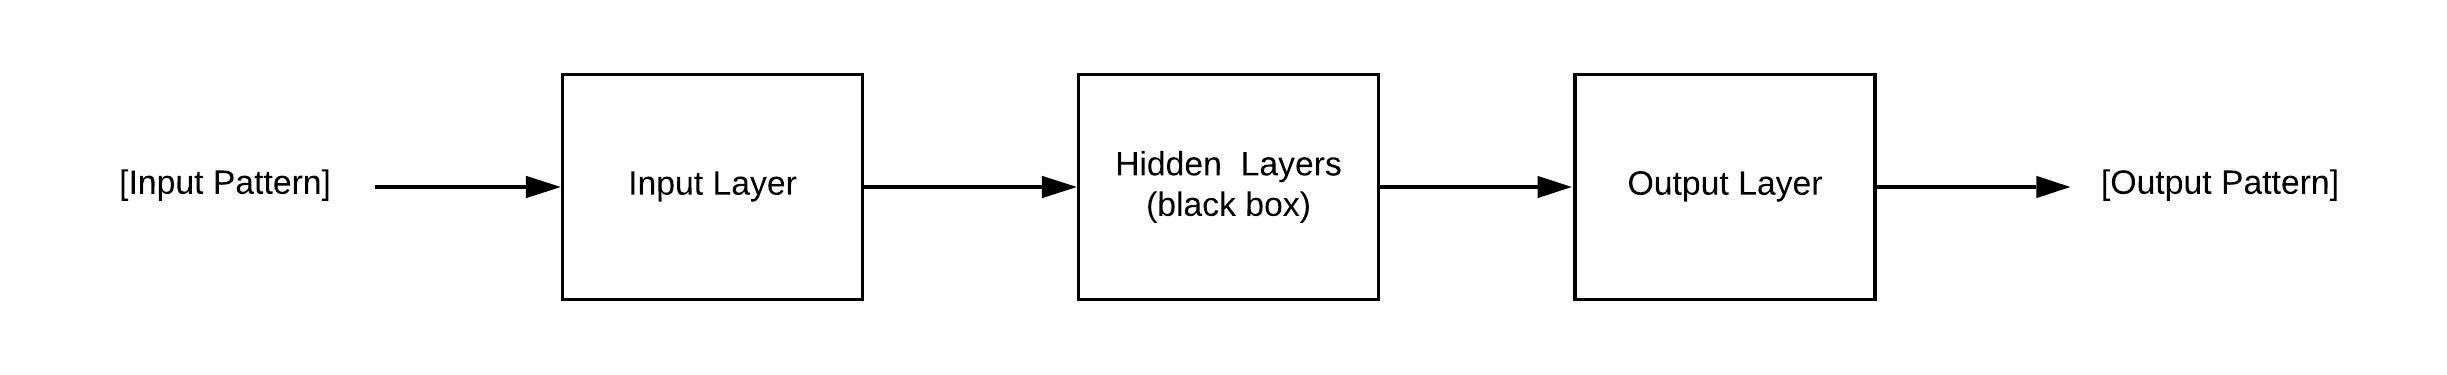
\includegraphics[width = 0.9\textwidth]{litreview/computervision/neuralnetworks/neural_network_basic_structure}
    \caption{Basic structure of a neural network \cite{neural_networks}.}
    \label{fig:neural_network}
\end{figure}

\subsubsection{Neurons}

The layers Neural networks are comprised of a fundamental unit called a neuron. Each neuron is comprised of an activiation function, a bias and a weight. An activiation function determines the output of a neuron as a function of its inputs, the simplest activation function is a step function, meaning that if the sum of the inputs is less than some threshold then the output of the neuron is 0, otherwise it's 1 \cite{machine_learning_dictionary}. A neuron's weight scales its output value when it's passed as an input to another neuron and thus alters the influence of a neuron's output on the entire neural network's output. A neuron's bias is a value that is added to the neuron's output. The bias is a trainable quantitiy meaning that it can be changed in order to change the behaviour of a neural network, however not all neural networks use biases \cite{neural_networks}. Figure \ref{fig:neuron} provides a diagram of a neuron outlining all of its components, inputs and outputs. 


\begin{figure}[h]
    \centering
    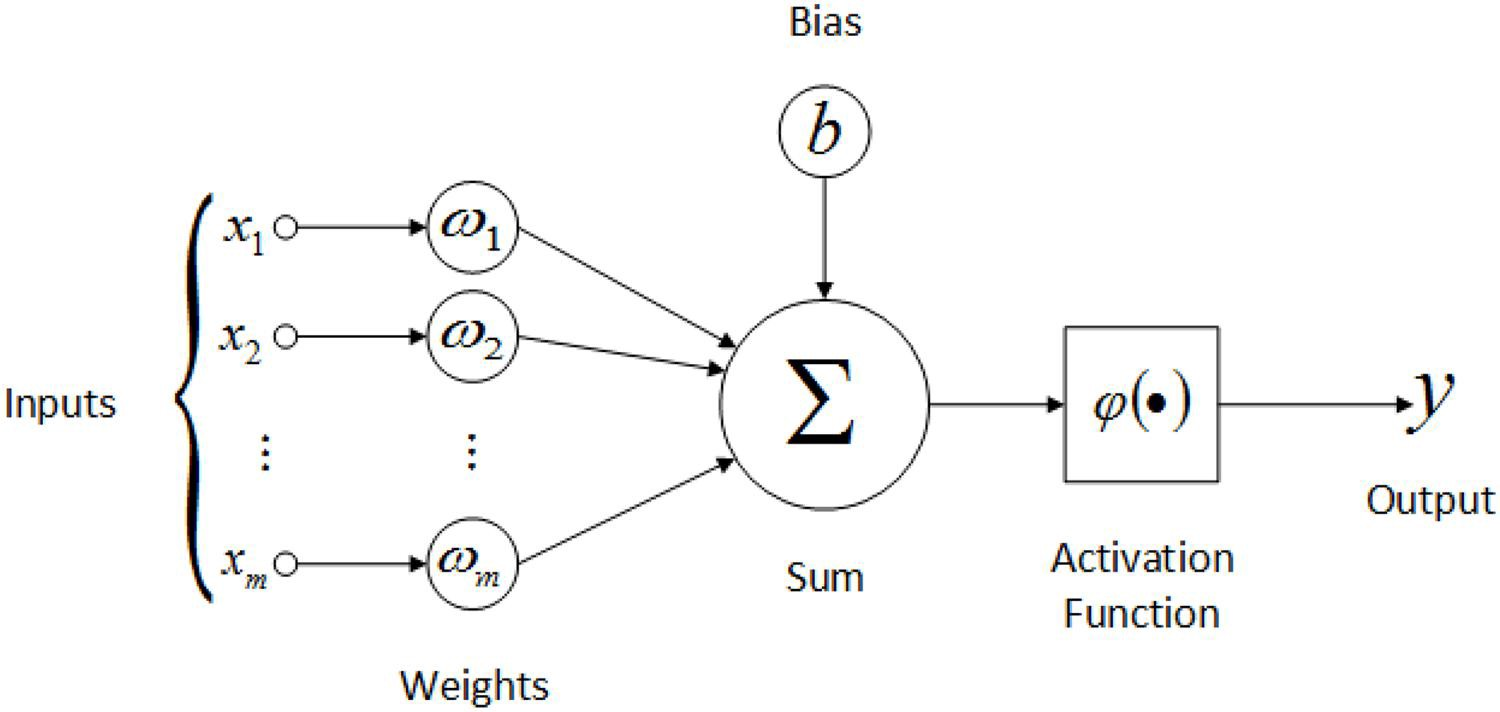
\includegraphics[width = 0.8\textwidth]{litreview/computervision/neuralnetworks/neuron}
    \caption{An artificial neuron \cite{ann_handbook}.}
    \label{fig:neuron}
\end{figure}

A single neuron on its own does not accomplish a lot however, given a large number of interacting neurons with weighting's and activiation function configured to recognise a specific pattern the desired output for a given input can be achieved.

\subsubsection{Data Aqcuisition and Training}

The process of determining the weightings of a neural network which in term determine its behaviour is achieved via \emph{training}. In training a neural network it is passed data samples and its response to them is observed, according to this response its weightings to improve the accuracy of its responses. All methods of network training require sample data test the network, for comprehensive computer vision applications in particular the amount of data required is very large \cite{large_data_neural_network}. The most successful neural networks are implemented with supervised learning algorithms meaning that they require labelled data, which can be costly in time or money \cite{patterns_machine_learning} \cite{supervised_neural_networks}. A sufficiently large amount of time must be spent collating and preparing data just to train a neural network \cite{data_labelling} that it can be regarded as disadvantage.

The execution of a training algorithm can also take a large amount of time dpeendent on the complexity of the network's activation functions and the amount of data required, these factors can make the requisite computation power to utilize a neural network, even after its trained, prohibitive for low power machines like microcontrollers \cite{computations_neural_network}. 

A simple method of evaluating a network's success at classifying data is to observe the ratio of successful classifications to unsuccessful ones. Evaluation becomes more complex when you consider not the absolute number of of classifications but the classification of individual data samples and whether or not they were correct. For a binary classification (just two classes) these measurements are referred to as true and false, positives and negatives \cite{neural_networks}. 


\section{Clustering}
Clustering is a method of segmenting an image into disjoint sets known as classes. This is useful for indentifying types of features or objects in an image. For example in Figure \ref{fig:toycar} the toy car has been identified out of the background.l

\begin{figure}[H]
	\centering
	\begin{subfigure}[b]{0.5\linewidth}
      		\centering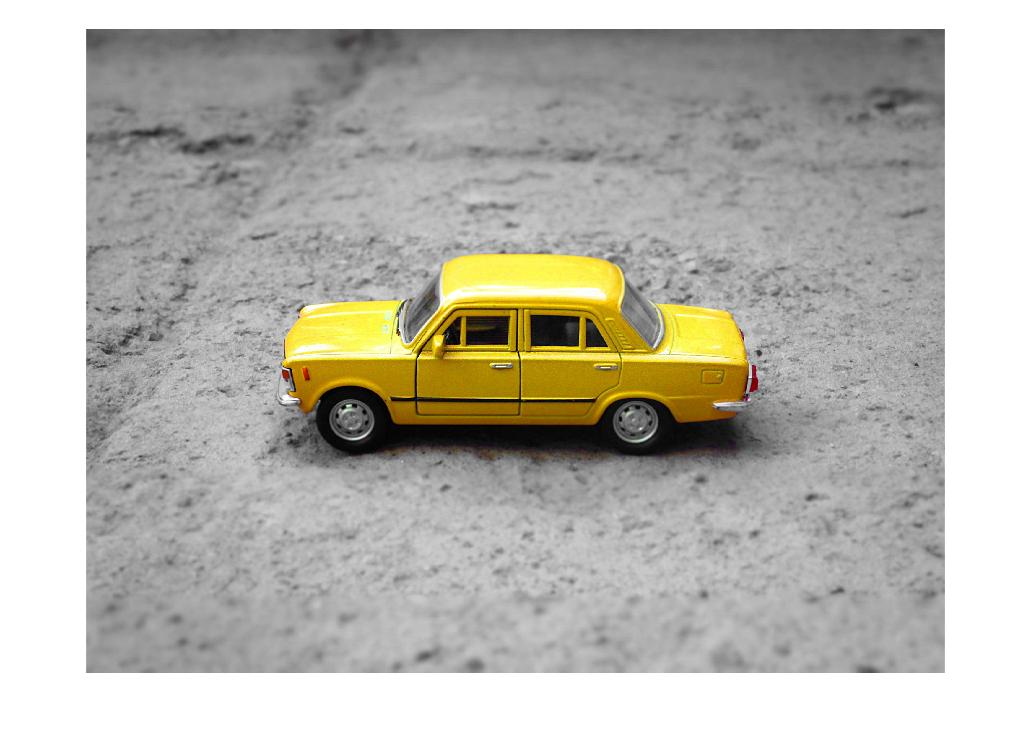
\includegraphics[width=220pt]{toyCar}
      		\caption{Image by Gustavo, Upsplash.}
		    \label{fig:toycarA}
    	\end{subfigure}%
    	\begin{subfigure}[b]{0.5\linewidth}
      		\centering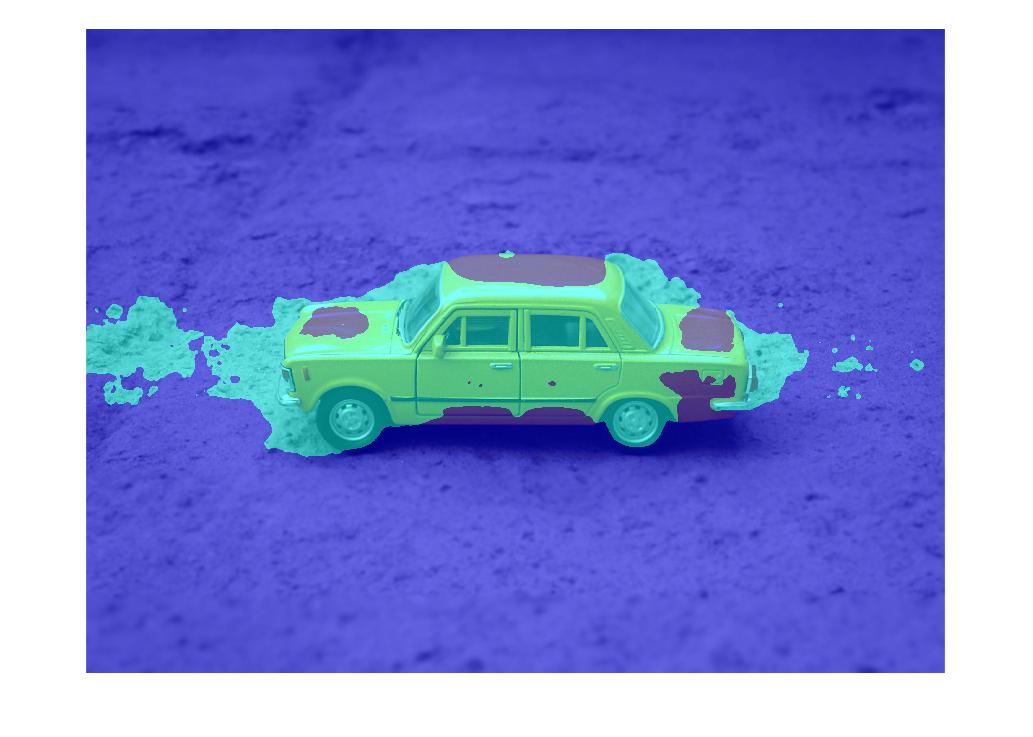
\includegraphics[width=220pt]{toycarseg}
      		\caption{Segmentation of car from background.}
       		\label{fig:toycarB}
    	\end{subfigure}
    	\caption{Segmentation of toy cars using K-Means Clustering.}
    	\label{fig:toycar}
\end{figure} 

In the context of an image generally every pixel is individually classified however groups of pixels known as superpixels may also be classified. Entities are classified based on the similarity of their features. For example, a pixel's intensity is a feature that could be used to cluster it with other pixels of similar intensity. As seen in (\ref{eq:featurevector}) an entity may be represented by any number of features, known also as dimensions, $d$. 

\begin{equation}
    \vec{v} = 
    \begin{bmatrix}
        d_1 \\
        d_2 \\
        \vdots \\ 
        d_n
    \end{bmatrix}
    \label{eq:featurevector}
\end{equation}



\subsubsection{K-Means}
\label{subsubsection:kmeans}
K-Means is simple and reasonably fast clustering algorithm where K represents the number of cluster the algorithm should create and means refers to the average value of each cluster. Given a set of data samples their similarity is measured as the value of the Euclidean distance between them. The general form of the Euclidean distance formula is described in equation \ref{eq:euclid}, where $p$ and $q$ represent n-dimensional feature vectors. As the K-means algorithm executes, data samples are assigned to the cluster whose average value, also as a cluster centroid, is closest to the sample's own. Centroids are updated after each round of assignments until their values converge. Initially the each cluster centroid is randomly selected. The algorithm to implement the K-means method is outlined in algorithm \ref{algorithm:kmeans}.

\begin{equation}
    EuclideanDistance(p,q) = \sqrt{(p_1 - q_1)^2 + (p_2 - q_2)^2 +\hdots + (p_n - q_n)^2}
    \label{eq:euclid}
\end{equation} 

\begin{algorithm}
    \SetAlgoLined
    \KwInput{Set of data vectors X of size M} 
    \KwOutput{K sets of clustered data vectors}
    Initialize the desired number of clusters $K$\;
    Initialize a list of $K$ random cluster centroids $\mu$\;
    \While{$\mu$ elements have not converged}{
        \For{i = 0 to M}
        {
            distOld = $\inf$
            \For{j = 0 to K}{
                distnew = EuclideanDistance(X[i], $\mu[j]$)\;
                \If{distNew $<$ distOld}{
                    distOld = distNew\;
                    $\mu_j$.append(X[i])\;
                }
            }
        }
        \For{p = 0 to K}{
            centroidList.append(average($\mu[p]$))\;
        }
    }
    \caption{K Means Clustering \cite{oreilly_python}}
    \label{algorithm:kmeans}
\end{algorithm}

The best result for this method is defined as having the smallest intra-cluster variance. K-Means is disadvantaged by the implicit trait that it formulates clusters of similar sizes. This happens because the algorithm seeks to minimize variance (spread) in each cluster hence the \q{ideal} centroid placement will form distributions spherically about centroids. Figure \ref{fig:clusters} visualizes an example of clustering data where it can be observed that the cluster sizes are similar and spherical in shape. This method of clustering does not consider any probabilistic model in classifying data, this type of classification is called a \emph{hard assignment} because a data sample can belong only to one cluster. The dual of this is a \emph{soft assignment}, considers the \emph{probability} of a sample of belonging each cluster. 

\begin{figure}[H]
    \centering
    \centering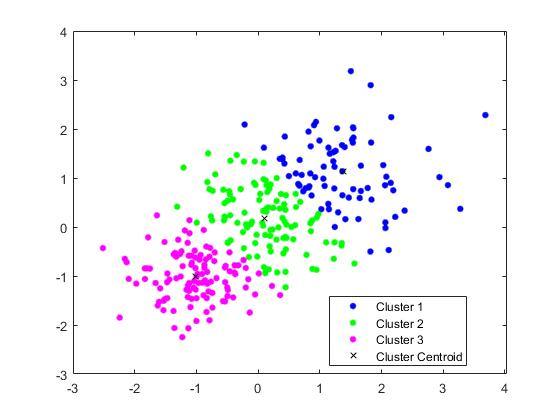
\includegraphics[width=0.9\textwidth]{kmeans_clusters}
    \caption{K-Means clustering performed on random data. \cite{matlab_clustering}}
    \label{fig:clusters}
\end{figure} 
\subsubsection{Mixtures of Gaussians}
 \label{subsection:mog}

Mixtures of Gaussians (MoG), or the Gaussian Mixture Model (GMM), is a method of clustering (see section \ref{subsection:clustering}) that is based not on distance \ref{subsubsection:kmeans} but distribution. This method of clustering was popularized by Duda and Hart in their text \emph{Pattern Classification and Scene Analysis} \cite{mog_seminal}. This method is more effective than distance based methods because it considers the covariance of the data. Note that for K-Means clustering the distributions were spherical, but if the true clusters were more elliptical then K-Means would fail to cluster them properly. Figure \ref{fig:cluster_shapes} compares what these cluster shapes might look like and the arrows indicate the location, the arrows indicate data points that are ambiguous.

\begin{figure}[h]
	\centering
	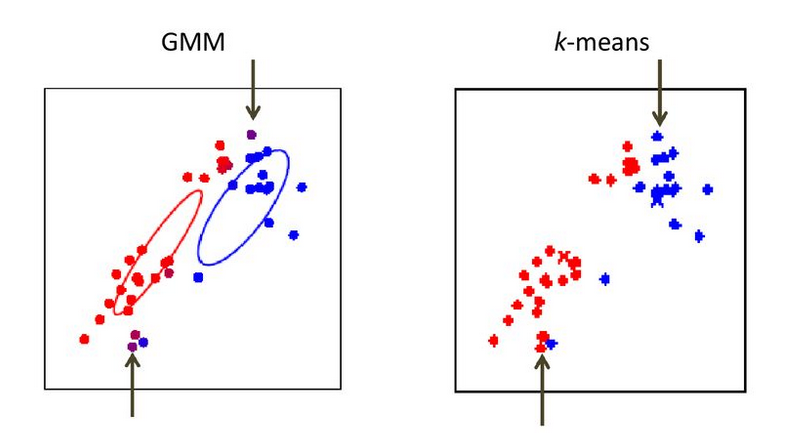
\includegraphics[width = 0.9\textwidth]{litreview/computervision/mog/mog_vs_kmeans.png}
	\captionsetup{format = hang}
	\caption{Comparison of K-Means cluster shape to GMM cluster shape. Img: Hongning Wang, University of Virginia }
	\label{fig:cluster_shapes}
\end{figure}
	
The basis of the Gaussian Mixture Model is of course the Gaussian Distribution function \ref{section:gaussian}. It is useful for probabilistic clustering because, as the Central Limit Theorem States, the distribution of the average value of the subsets of any data set will approximately converge to a Normal distribution as the number of terms in the subsets increases \cite{patterns_machine_learning}. The Mixture of Gaussian for the random variable $\boldsymbol{x}$ is achieved by super-positioning the distributions of random variable for each cluster. Equation \ref{eq:mog} describes the super-positioning of $K$ distributions for random variable $\boldsymbol{x}$, the resulting curve models the distribution of the random variable. 

\begin{equation}
p(\boldsymbol{x}) = \sum^{K}_{k = 1}\pi_k \mathcal{N}(\boldsymbol{x}|\boldsymbol{\mu_k}, \boldsymbol{\Sigma_k})
\label{eq:mog}
\end{equation}

The variable $\pi_k$ is known as the \emph{mixing coefficient} of a Gaussian distribution which controls the weighting of a particular distribution in the mixture. The sum of the mixing ratios is 1 because the complete mixture distribution represent the probability of a sample belonging to any one cluster and it must belong to one, hence

\[\sum_{k=1}^K\pi_k = 1\]

To help to understand how equation \ref{eq:mog} came about consider the random variable $\boldsymbol{z}$ of dimension K which is a binary random variable, meaning it can only have value 1 or 0. Only one element of $\boldsymbol{z}$ can be equal to 1 and all others must be 0, thus

\[\sum_{k=1}^Kz_k = 1\]

Hence there are K possible combinations of the vector $\boldsymbol{z}$. The marginal distribution over $\boldsymbol{z}$ is defined in terms of the mixing coefficients, 

\[p(z_k = 1) = \pi_k\]

That is to say the probability of $z_k$ = 1 is equal to the mixing coefficient of Gaussian distribution k. This can also be written

\[p(\boldsymbol{z}) = \prod^K_{k=1}\pi^{z_k}_k\]

The significance of $\boldsymbol{z}$ represents the assignment of a sample to a cluster which is why only one of its elements can be 1. To observe the Gaussian distribution of $\boldsymbol{z}$ in cluster $K$ we set $z_k = 1$ as described by the condition distribution,

\[p(\bm{x}|\boldsymbol{z}) = \mathcal{N}(\boldsymbol{x}|\boldsymbol{\mu_k}, \boldsymbol{\Sigma_k}) \]

Finally we can determine that the marginal distribution of $\boldsymbol{z}$ which is described by \ref{eq:mog} using the marginal distribution $p(\boldsymbol{z})$ and the conditional distribution $p(\bm{x}|\bm{z})$ as 

\begin{align}
	p(\bm{x}) 	&= p(\bm{z})p(\bm{x}|\bm{z})
				&= \sum^{K}_{k = 1}\pi_k \mathcal{N}(\boldsymbol{x}|\boldsymbol{\mu_k}, \boldsymbol{\Sigma_k})
\label{eq:mog_derive}
\end{align}

Figure \ref{fig:mog_compare}

\begin{figure}[htbp]
    \centering
     \begin{subfigure}[b]{0.45\textwidth}
        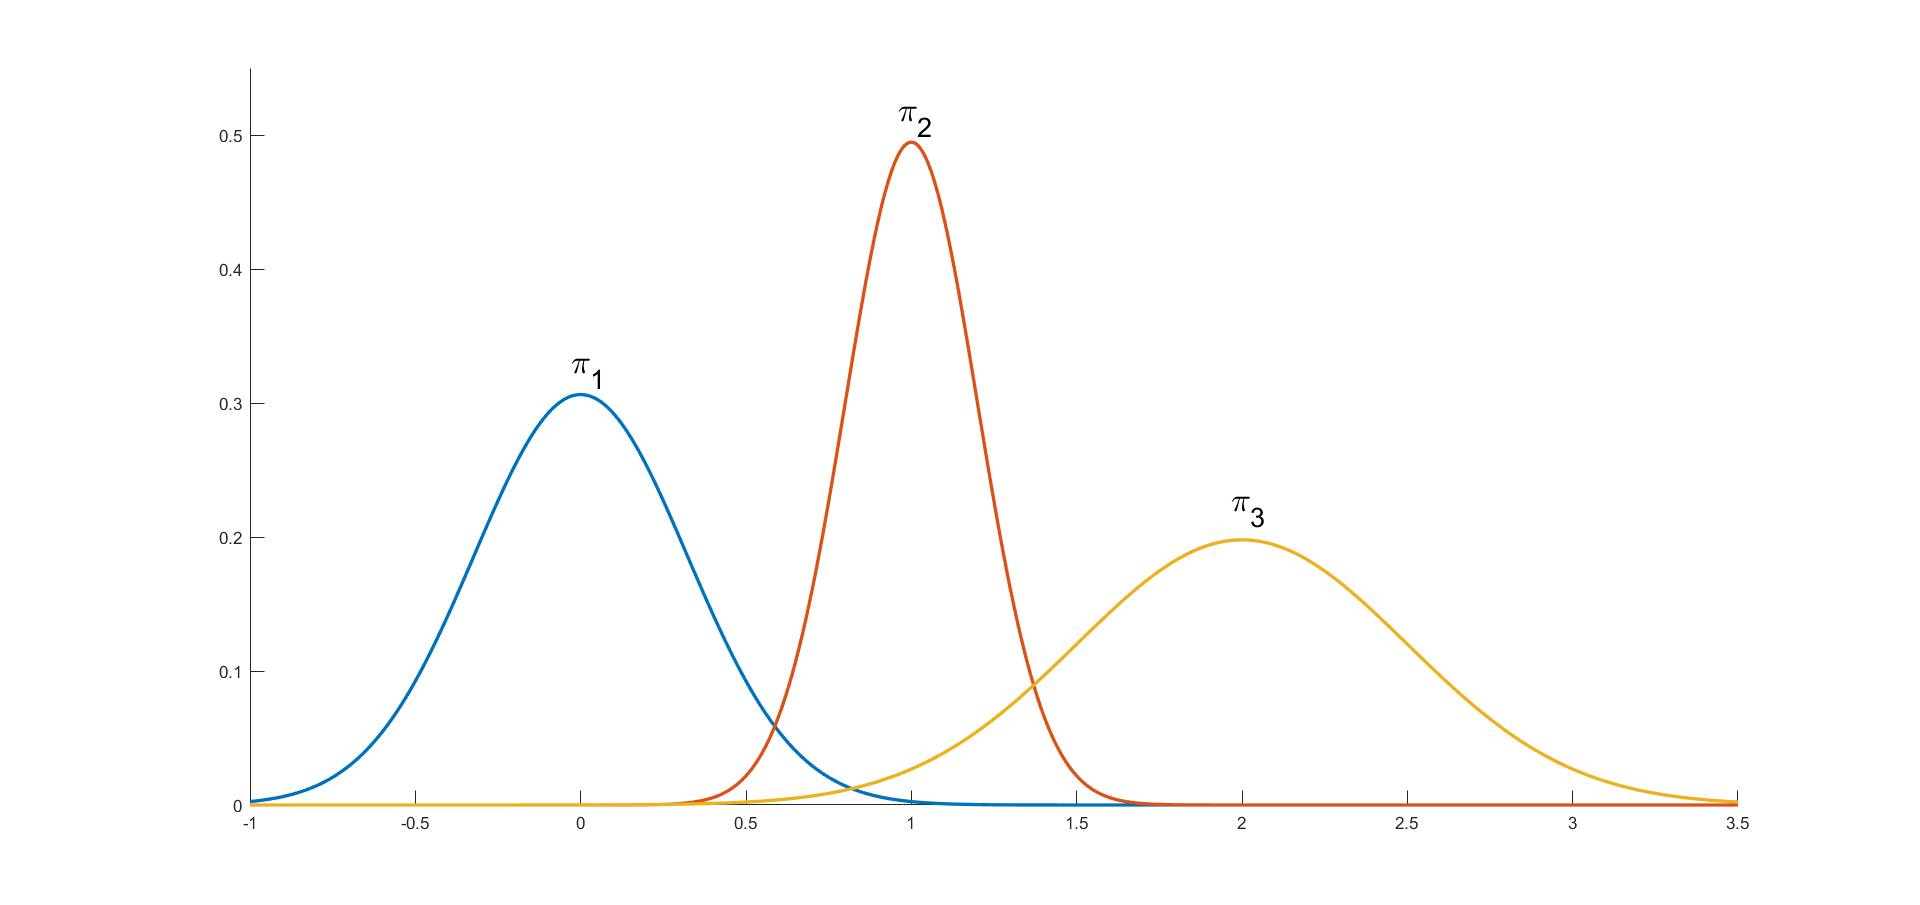
\includegraphics[width=\textwidth]{litreview/machinelearning/clustering/mog/individual_gauss.png}
	\captionsetup{format = hang}
        \caption{Three individual cluster distributions.}
        \label{fig:mog_singles}
    \end{subfigure} 
    \begin{subfigure}[b]{0.45\textwidth}
        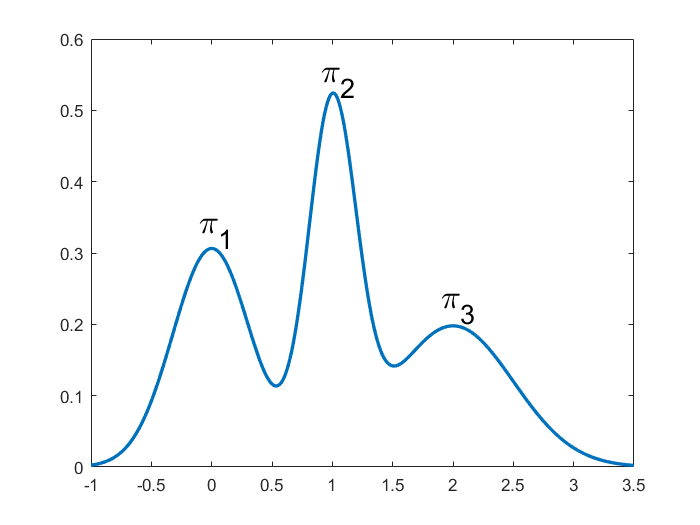
\includegraphics[width=\textwidth]{litreview/machinelearning/clustering/mog/combined_mog.png}	
	\captionsetup{format = hang}
        \caption{Super-positioned Gaussian distributions}
        \label{fig:mog_combined}
    \end{subfigure}
    \captionsetup{format = hang}
    \caption{Visualization of a Mixture of Gaussians for 1D dataset.}
    \label{fig:mog_compare}
\end{figure}











Initially, K Gaussian functions are randomly generated corresponding to K clusters. If a dataset has low dimensionality, by taking a histogram of its values the Gaussians' initial conditions can be approximated, as in Figure \ref{fig:histGauss}. By super-positioning all of the Gaussians a sample's complete probabilistic model is created, i.e. a model for \emph{all} clusters, see Figure \ref{fig:histCurve}. 

\begin{figure}[H]
	\centering
	\begin{subfigure}[b]{0.5\linewidth}
            \centering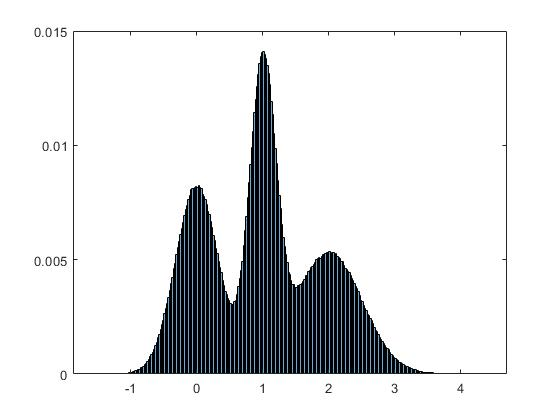
\includegraphics[width=215pt]{histGauss}
      		\caption{Normalized Histogram of 1D samples.}
		\label{fig:histGauss}
    	\end{subfigure}%
    	\begin{subfigure}[b]{0.5\linewidth}
      		\centering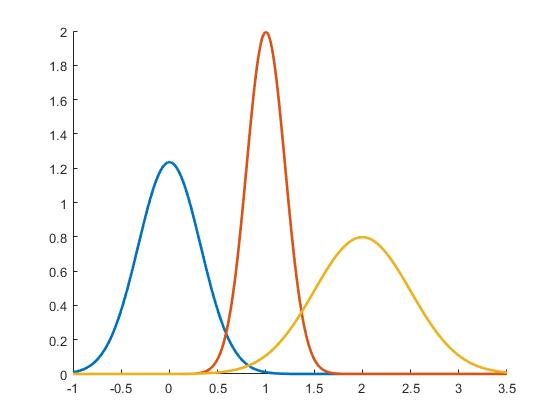
\includegraphics[width=215pt]{hist_gauss_curve}
      		\caption{Gaussians derived from 1D histogram.}
       		\label{fig:histCurve}
		\end{subfigure}
		\caption{Formulation of Mixture of Gaussians.}
    	\label{fig:mixture}
\end{figure}

With each iteration of the GMM algorithm the parameters of the model's component Gaussians are tuned according to the covariance between samples in each cluster. In \ref{eq:cov} $X$ and $Y$ are the variables being compared, $\overline X$ and $\overline Y$ are variable means and $n$ is the number of samples. For a multidimensional dataset a covariance matrix $\bm{\Sigma_k}$ will be generated and each Gaussian will require a mean vector $\bm{\mu_k}$ as opposed to a scalar. 

\begin{equation}
Cov(X, Y) = \frac{\Sigma(X_i-\overline X)(Y_j-\overline Y)}{n}
\label{eq:cov}
\end{equation}



The algorithm seeks the highest covariance possible in each of its clusters. It is by considering the covariance of samples that the GMM is able to best classify ambiguous samples. The higher the covariance (aka correlation) between sample dimensions the more likely it is they belong in the same cluster. This can observed in Figure \ref{fig:mogcov}, the data being clustered is the same as in Figure \ref{fig:clusters} but notice the elliptical shape of the Gaussian cluster distributions as opposed to the spherical shape of K-Means clustering.

\begin{figure}[H]
	\centering
	\centering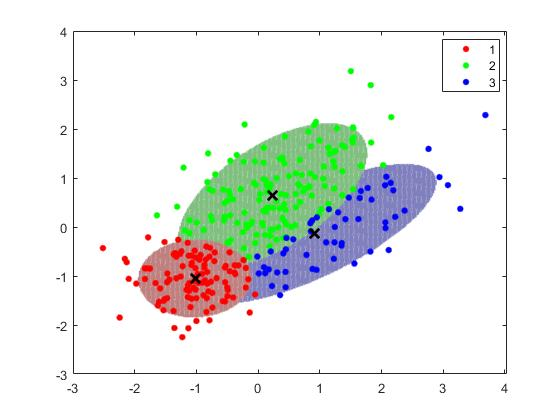
\includegraphics[width=450pt]{mog}
	\caption{Clustering using GMM. X marks cluster mean.}
	\label{fig:mogcov}
\end{figure}
  
In Figure \ref{fig:histScale} the Gaussians from Figure \ref{fig:histCurve} have been scaled to have the amplitudes $\pi_1 = 0.3$, $\pi_1 = 0.5$ and $\pi_1 = 0.2$. These are weightings that give the mixing ratio of the GMM and represent each cluster's proportion of the total samples. The more samples a cluster contains the more likely it is a sample belongs to it. The sum of ratios must add to one because the probability a sample belongs to at least one cluster is one, as defined in \ref{eq:gauss_weight1} and \ref{eq:gauss_weight2}.

\begin{equation}
    0\leq \pi_k \leq 1
\label{eq:gauss_weight1}
\end{equation}
\begin{equation}
    \sum_{k=1}^{K}\pi_k = 1
\label{eq:gauss_weight2}
\end{equation}


\begin{figure}[H]
    \centering
    \centering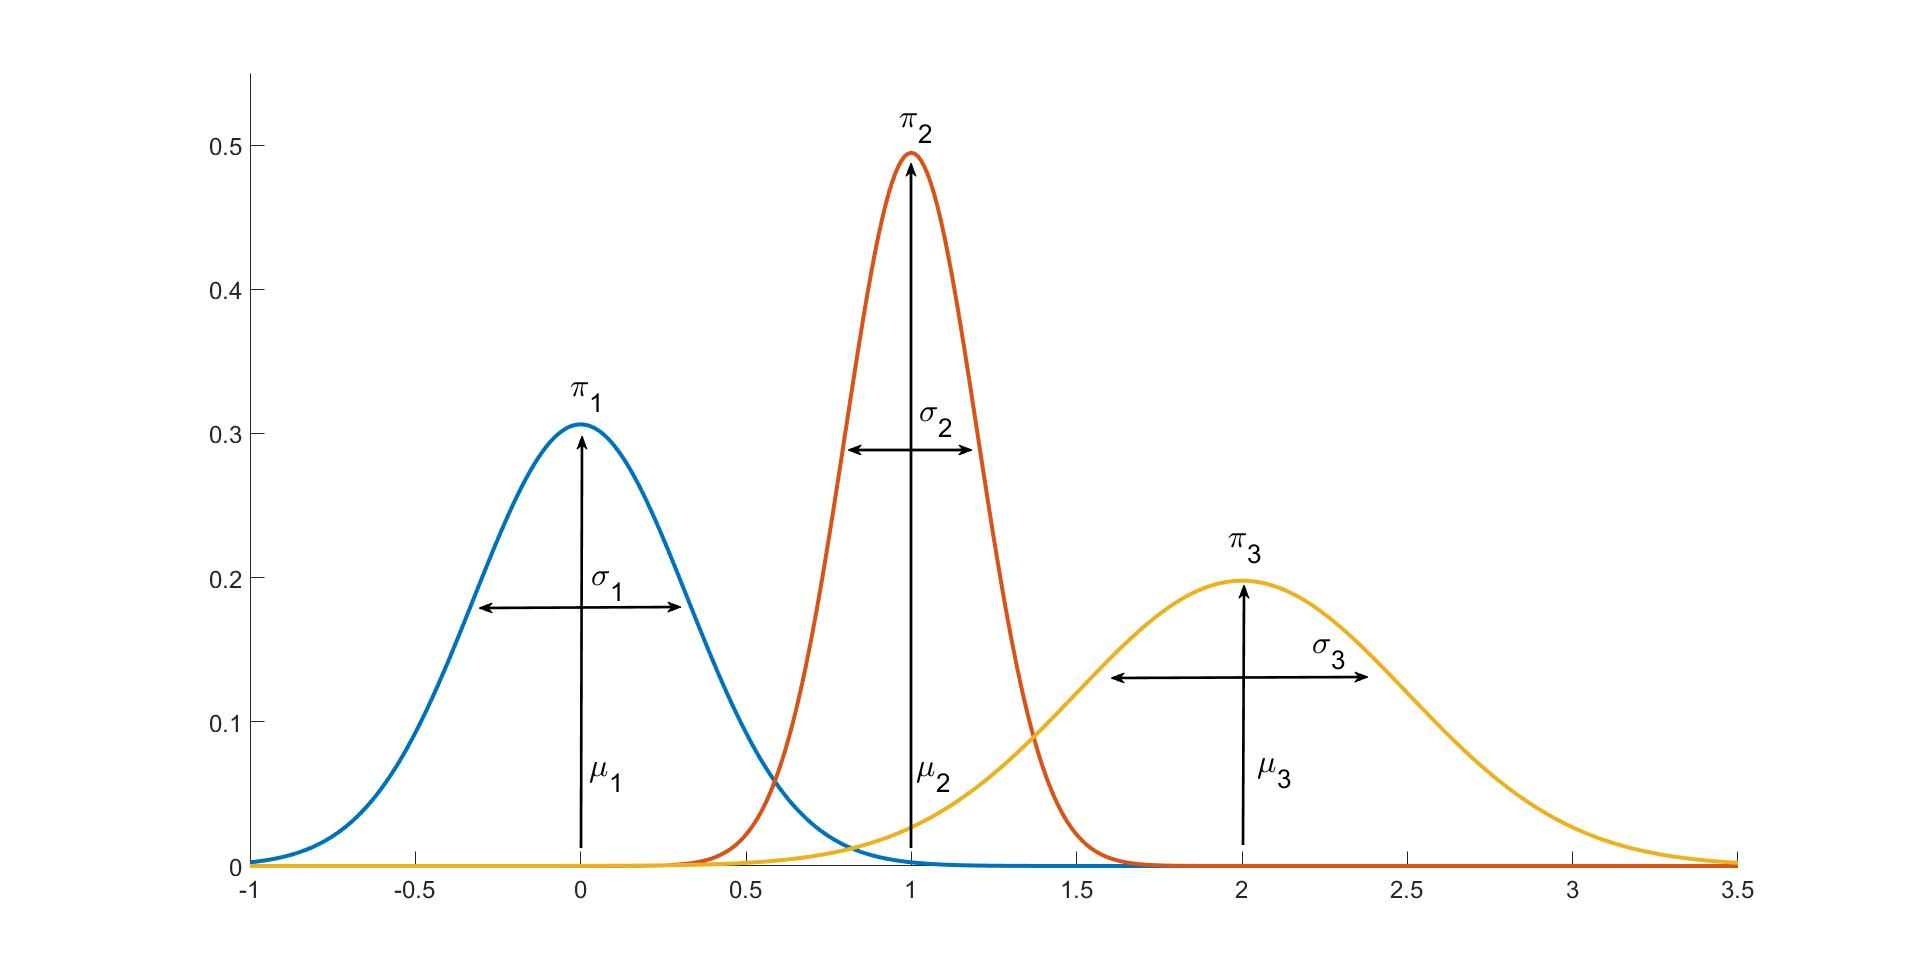
\includegraphics[width=450pt]{gauss_mix_scale}
    \caption{Individual Gaussians with scaled weightings.}
    \label{fig:histScale}
  \end{figure} 

Each Gaussian's three parameters, mean $\bm{\mu}_k$, ampltidue $\pi_k$ and covariance $\bm{\Sigma}_k$ are updated following each iteration of the algorithm according to the 'Expectation Maximization' algorithm.

\subsubsection{Expectation Maximization}

Expectation Maximization (EM) is a method of updating the parameters of cluster Gaussians that seeks to maximize a sample's likelihood of belonging to said Gaussians (\ref{eq:likelihood}). 

\begin{equation}
\label{eq:likelihood}
p(x) = \sum^K_{k=1} \pi_k \mathcal{N}(x|\bm{\mu}_k, \bm{\Sigma}_k)
\end{equation}

A binary indicator $z_{i}$ exists for every sample $x_i$, it is 1 if the sample belongs in the cluster $k$ and 0 otherwise such that $z_{ik} \in \{0, 1\}$ and $\sum_k z_{ik} = 1$. If the data is multidimensional then the sample and inidicator are both vectors, $\bm{x}$ and $\bm{z}$. The marginal probability $p(\bm{z}_{k} = 1)$ is the probability that a sample $\bm{x}$ is in cluster $k$. This quantity is completely specified by the mixture weight $\pi_k$ for each Gaussian because the area under a Gaussian component is equal to its mixing ratio, i.e.

\begin{equation}
	\label{eq:marginalk}
	p(\bm{z}_{k}=1) = \pi_k 
\end{equation}
	
If we know that a sample $\bm{x}$ is from cluster $k$ the \emph{likelihood} of seeing it in the associated Gaussian is the value of the Gaussian at that point,
\begin{equation}
	\label{eq:cond}
	p(\bm{x}\, |\, \bm{z}_{k} = 1) = \mathcal{N}(\bm{x}\, |\,\bm{\mu_k}, \bm{\Sigma_k})
\end{equation}

The conditional probability of $\bm{z}_{ik}$ given the value of sample, $\bm{x}_i$ is denoted as $\gamma(\bm{z}_{ik})$. This is the probability that a sample belongs to cluster $k$ given its value $\bm{x}_i$ and is the quantity of interest when trying to classify a sample.  Using Bayes Theorem [REF APPENDIX] quantity can be found 

\begin{align}
	\gamma(\bm{z}_{ik}) \equiv p(\bm{z}_{ik} =1 | \bm{x}_i)
	\label{eq:gamma2}
	&= \frac{p(\bm{z}_{ik}=1)p(\bm{x}_i\, |\, \bm{z}_{ik} = 1)}{\sum^K_{j=1}p(\bm{z}_{jk}=1)p(\bm{x}_j\, |\, \bm{z}_{jk} = 1)}\\ 
	\label{eq:gamma3}
	&= \frac{\pi_k\, \mathcal{N}(\bm{x}\,|\,\bm{\mu_k},\bm{\Sigma_k})}{\sum_{j=1}^{K}\pi_k\, \mathcal{N}(\bm{x}\,|\,\bm{\mu_k},\bm{\Sigma_k})}
\end{align}


To maximize the likelihood of each sample being in each Gaussian the distribution parameters are modified. This is achieved by taking derivatives of the log of the likelihood function (\ref{eq:likelihood}) with respect to each Gaussian parameter and setting the result to 0 to find local maxima. To take the log of the likelihood function assume all samples in are in an $N \times D$ matrix $\bm{X}$ and the corresponding indicators are in an $ N \times K$ matrix $\bm{Z}$. 

\begin{equation}
\label{eq:log}
ln\,p(X|\bm{\pi}, \bm{\mu}, \bm{\Sigma}) = \sum_{n=1}^N
ln \Bigg\{ \sum_{k=1}^K \pi_k\mathcal(N)(\bm{x}_n|\bm{\mu}_k,\bm{\Sigma}_k)\Bigg\}
\end{equation}







\centerline{}

The EM algorithm is comprised of [X] steps

%% EM STEPS %%
\begin{enumerate}
	\item Generate the initial K Gaussian parameters mean $\bm{\mu}_{k}$, covariance $\bm{\Sigma}_k$ and mixing ratios $\pi_k$ either randomly or informed by a histogram.
	\item Estimate the likelihood sample n was generated by cluster k for all samples. 
	\begin{equation}
		\gamma(\bm{z}_{ik})=\frac{\pi_k\, \mathcal{N}(\bm{x}\,|\,\bm{\mu_k},\bm{\Sigma_k})}{\sum_{j=1}^{K}\pi_k\, \mathcal{N}(\bm{x}\,|\,\bm{\mu_k},\bm{\Sigma_k})}
	\end{equation}

	\item Maximize the Gaussian parameter using derivatives of log likelihood for each parameter.
	\begin{align}	
	\label{eq:mean}
	\bm{\mu}_{k}^{new} &= \frac{1}{N_k}\sum_{n=1}^N \gamma(z_{nk} ) \bm{x}_n \\
	\label{eq:covariance}
	\bm{\Sigma}_k^{new} &=  \frac{1}{N_k}\sum_{n=1}^N\gamma(z_{nk})(\bm{x}_n- \bm{\mu}_k^{new})(\bm{x}_n - \bm{\mu}_k^{new})^T \\
	\label{eq:ratio}
	\pi_k &= \frac{N_k}{N}
	\end{align}
	where \newline
	\[N_k = \sum_{i} z_{ik}\]
	\item Repeat steps 2 and 3 until convergence of log likelihood (\ref{eq:likelihood}) or parameters. 
\end{enumerate}

The Gaussian Mixture Model method of clustering is computationally complex compared to K-Means however it's ability to differentiate ambiguous samples by considering covariance is superior. 



\subsubsection{Mixtures of Gaussians}
 \label{subsection:mog}

Mixtures of Gaussians (MoG), or the Gaussian Mixture Model (GMM), is a method of clustering (see section \ref{subsection:clustering}) that is based not on distance \ref{subsubsection:kmeans} but distribution. This method of clustering was popularized by Duda and Hart in their text \emph{Pattern Classification and Scene Analysis} \cite{mog_seminal}. This method is more effective than distance based methods because it considers the covariance of the data. Note that for K-Means clustering the distributions were spherical, but if the true clusters were more elliptical then K-Means would fail to cluster them properly. Figure \ref{fig:cluster_shapes} compares what these cluster shapes might look like and the arrows indicate the location, the arrows indicate data points that are ambiguous.

\begin{figure}[h]
	\centering
	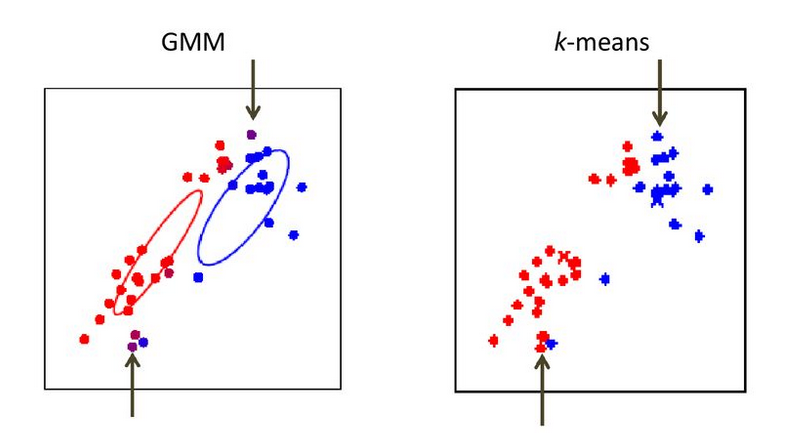
\includegraphics[width = 0.9\textwidth]{litreview/computervision/mog/mog_vs_kmeans.png}
	\captionsetup{format = hang}
	\caption{Comparison of K-Means cluster shape to GMM cluster shape. Img: Hongning Wang, University of Virginia }
	\label{fig:cluster_shapes}
\end{figure}
	
The basis of the Gaussian Mixture Model is of course the Gaussian Distribution function \ref{section:gaussian}. It is useful for probabilistic clustering because, as the Central Limit Theorem States, the distribution of the average value of the subsets of any data set will approximately converge to a Normal distribution as the number of terms in the subsets increases \cite{patterns_machine_learning}. The Mixture of Gaussian for the random variable $\boldsymbol{x}$ is achieved by super-positioning the distributions of random variable for each cluster. Equation \ref{eq:mog} describes the super-positioning of $K$ distributions for random variable $\boldsymbol{x}$, the resulting curve models the distribution of the random variable. 

\begin{equation}
p(\boldsymbol{x}) = \sum^{K}_{k = 1}\pi_k \mathcal{N}(\boldsymbol{x}|\boldsymbol{\mu_k}, \boldsymbol{\Sigma_k})
\label{eq:mog}
\end{equation}

The variable $\pi_k$ is known as the \emph{mixing coefficient} of a Gaussian distribution which controls the weighting of a particular distribution in the mixture. The sum of the mixing ratios is 1 because the complete mixture distribution represent the probability of a sample belonging to any one cluster and it must belong to one, hence

\[\sum_{k=1}^K\pi_k = 1\]

To help to understand how equation \ref{eq:mog} came about consider the random variable $\boldsymbol{z}$ of dimension K which is a binary random variable, meaning it can only have value 1 or 0. Only one element of $\boldsymbol{z}$ can be equal to 1 and all others must be 0, thus

\[\sum_{k=1}^Kz_k = 1\]

Hence there are K possible combinations of the vector $\boldsymbol{z}$. The marginal distribution over $\boldsymbol{z}$ is defined in terms of the mixing coefficients, 

\[p(z_k = 1) = \pi_k\]

That is to say the probability of $z_k$ = 1 is equal to the mixing coefficient of Gaussian distribution k. This can also be written

\[p(\boldsymbol{z}) = \prod^K_{k=1}\pi^{z_k}_k\]

The significance of $\boldsymbol{z}$ represents the assignment of a sample to a cluster which is why only one of its elements can be 1. To observe the Gaussian distribution of $\boldsymbol{z}$ in cluster $K$ we set $z_k = 1$ as described by the condition distribution,

\[p(\bm{x}|\boldsymbol{z}) = \mathcal{N}(\boldsymbol{x}|\boldsymbol{\mu_k}, \boldsymbol{\Sigma_k}) \]

Finally we can determine that the marginal distribution of $\boldsymbol{z}$ which is described by \ref{eq:mog} using the marginal distribution $p(\boldsymbol{z})$ and the conditional distribution $p(\bm{x}|\bm{z})$ as 

\begin{align}
	p(\bm{x}) 	&= p(\bm{z})p(\bm{x}|\bm{z})
				&= \sum^{K}_{k = 1}\pi_k \mathcal{N}(\boldsymbol{x}|\boldsymbol{\mu_k}, \boldsymbol{\Sigma_k})
\label{eq:mog_derive}
\end{align}

Figure \ref{fig:mog_compare}

\begin{figure}[htbp]
    \centering
     \begin{subfigure}[b]{0.45\textwidth}
        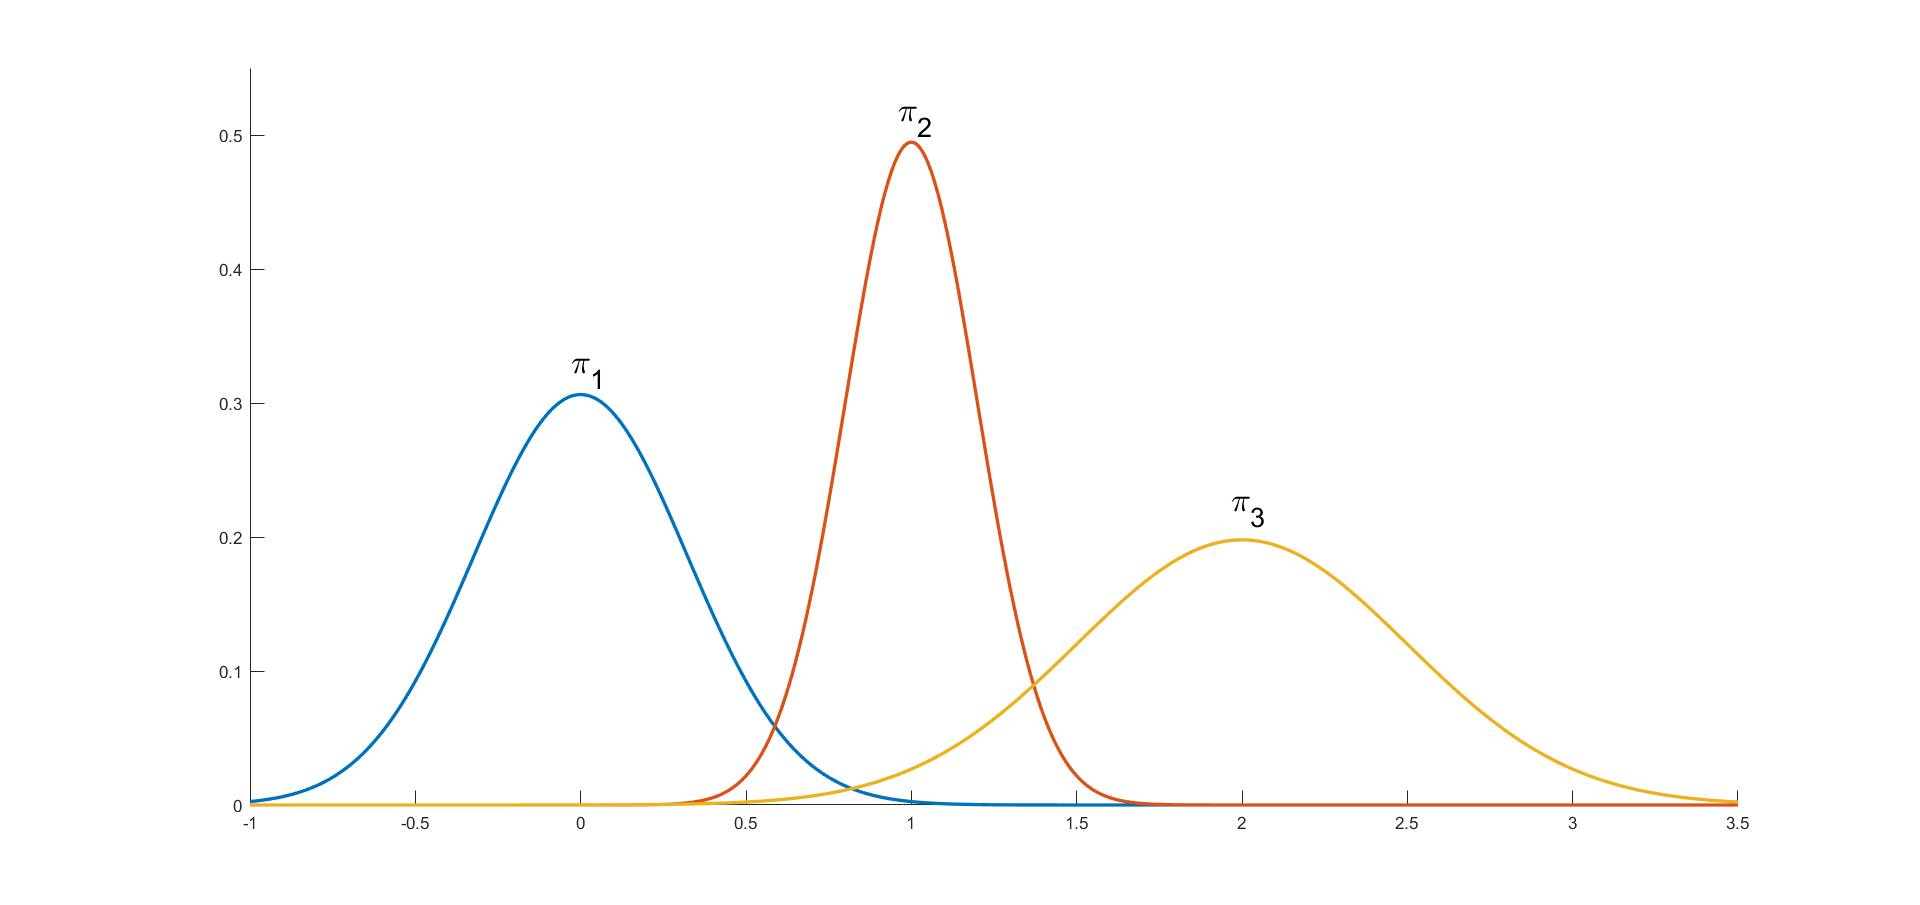
\includegraphics[width=\textwidth]{litreview/machinelearning/clustering/mog/individual_gauss.png}
	\captionsetup{format = hang}
        \caption{Three individual cluster distributions.}
        \label{fig:mog_singles}
    \end{subfigure} 
    \begin{subfigure}[b]{0.45\textwidth}
        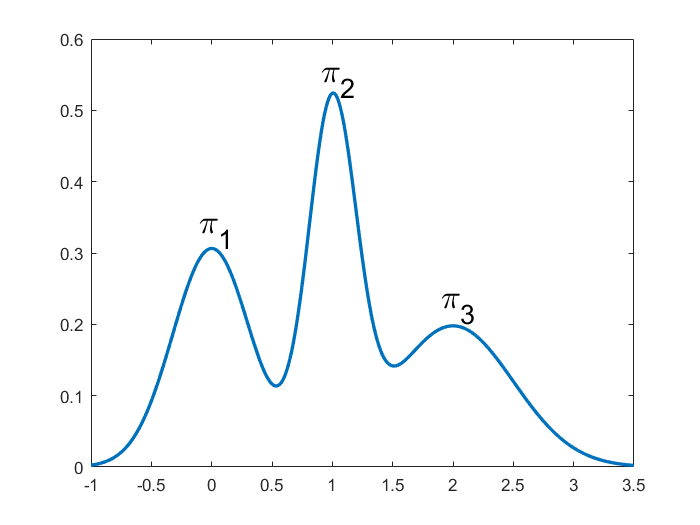
\includegraphics[width=\textwidth]{litreview/machinelearning/clustering/mog/combined_mog.png}	
	\captionsetup{format = hang}
        \caption{Super-positioned Gaussian distributions}
        \label{fig:mog_combined}
    \end{subfigure}
    \captionsetup{format = hang}
    \caption{Visualization of a Mixture of Gaussians for 1D dataset.}
    \label{fig:mog_compare}
\end{figure}











Initially, K Gaussian functions are randomly generated corresponding to K clusters. If a dataset has low dimensionality, by taking a histogram of its values the Gaussians' initial conditions can be approximated, as in Figure \ref{fig:histGauss}. By super-positioning all of the Gaussians a sample's complete probabilistic model is created, i.e. a model for \emph{all} clusters, see Figure \ref{fig:histCurve}. 

\begin{figure}[H]
	\centering
	\begin{subfigure}[b]{0.5\linewidth}
            \centering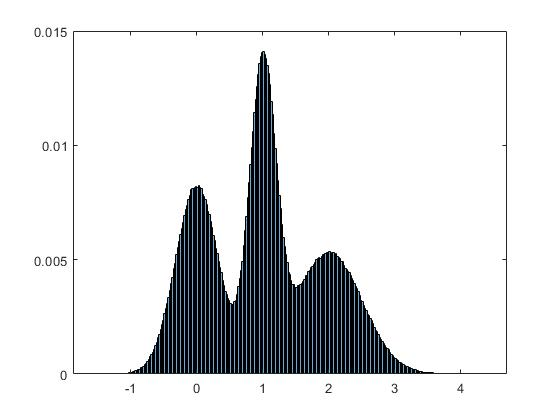
\includegraphics[width=215pt]{histGauss}
      		\caption{Normalized Histogram of 1D samples.}
		\label{fig:histGauss}
    	\end{subfigure}%
    	\begin{subfigure}[b]{0.5\linewidth}
      		\centering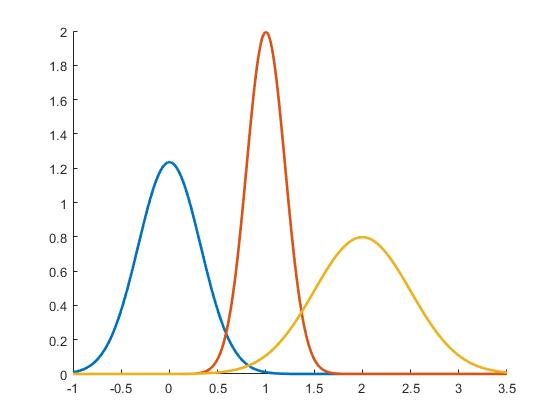
\includegraphics[width=215pt]{hist_gauss_curve}
      		\caption{Gaussians derived from 1D histogram.}
       		\label{fig:histCurve}
		\end{subfigure}
		\caption{Formulation of Mixture of Gaussians.}
    	\label{fig:mixture}
\end{figure}

With each iteration of the GMM algorithm the parameters of the model's component Gaussians are tuned according to the covariance between samples in each cluster. In \ref{eq:cov} $X$ and $Y$ are the variables being compared, $\overline X$ and $\overline Y$ are variable means and $n$ is the number of samples. For a multidimensional dataset a covariance matrix $\bm{\Sigma_k}$ will be generated and each Gaussian will require a mean vector $\bm{\mu_k}$ as opposed to a scalar. 

\begin{equation}
Cov(X, Y) = \frac{\Sigma(X_i-\overline X)(Y_j-\overline Y)}{n}
\label{eq:cov}
\end{equation}



The algorithm seeks the highest covariance possible in each of its clusters. It is by considering the covariance of samples that the GMM is able to best classify ambiguous samples. The higher the covariance (aka correlation) between sample dimensions the more likely it is they belong in the same cluster. This can observed in Figure \ref{fig:mogcov}, the data being clustered is the same as in Figure \ref{fig:clusters} but notice the elliptical shape of the Gaussian cluster distributions as opposed to the spherical shape of K-Means clustering.

\begin{figure}[H]
	\centering
	\centering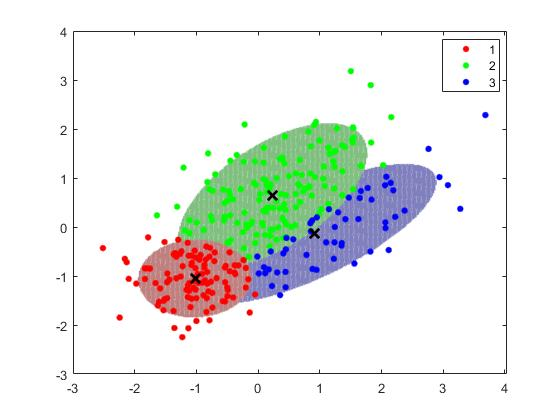
\includegraphics[width=450pt]{mog}
	\caption{Clustering using GMM. X marks cluster mean.}
	\label{fig:mogcov}
\end{figure}
  
In Figure \ref{fig:histScale} the Gaussians from Figure \ref{fig:histCurve} have been scaled to have the amplitudes $\pi_1 = 0.3$, $\pi_1 = 0.5$ and $\pi_1 = 0.2$. These are weightings that give the mixing ratio of the GMM and represent each cluster's proportion of the total samples. The more samples a cluster contains the more likely it is a sample belongs to it. The sum of ratios must add to one because the probability a sample belongs to at least one cluster is one, as defined in \ref{eq:gauss_weight1} and \ref{eq:gauss_weight2}.

\begin{equation}
    0\leq \pi_k \leq 1
\label{eq:gauss_weight1}
\end{equation}
\begin{equation}
    \sum_{k=1}^{K}\pi_k = 1
\label{eq:gauss_weight2}
\end{equation}


\begin{figure}[H]
    \centering
    \centering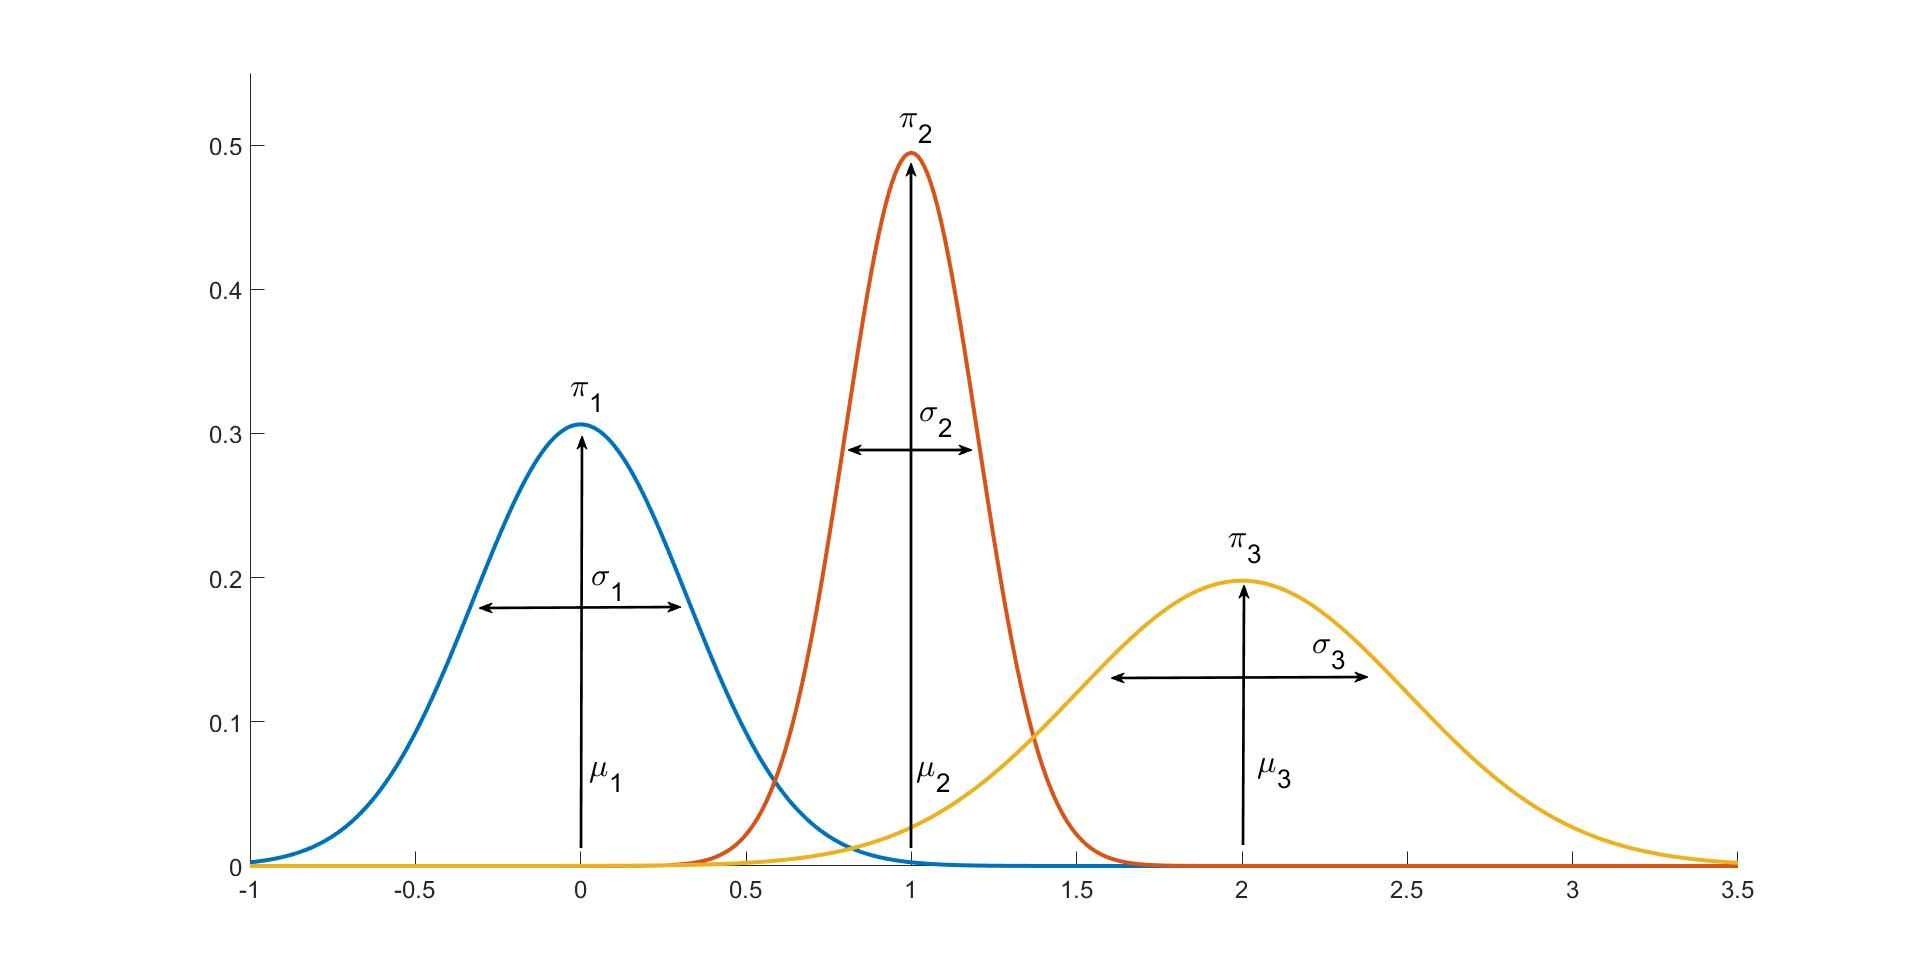
\includegraphics[width=450pt]{gauss_mix_scale}
    \caption{Individual Gaussians with scaled weightings.}
    \label{fig:histScale}
  \end{figure} 

Each Gaussian's three parameters, mean $\bm{\mu}_k$, ampltidue $\pi_k$ and covariance $\bm{\Sigma}_k$ are updated following each iteration of the algorithm according to the 'Expectation Maximization' algorithm.

\subsubsection{Expectation Maximization}

Expectation Maximization (EM) is a method of updating the parameters of cluster Gaussians that seeks to maximize a sample's likelihood of belonging to said Gaussians (\ref{eq:likelihood}). 

\begin{equation}
\label{eq:likelihood}
p(x) = \sum^K_{k=1} \pi_k \mathcal{N}(x|\bm{\mu}_k, \bm{\Sigma}_k)
\end{equation}

A binary indicator $z_{i}$ exists for every sample $x_i$, it is 1 if the sample belongs in the cluster $k$ and 0 otherwise such that $z_{ik} \in \{0, 1\}$ and $\sum_k z_{ik} = 1$. If the data is multidimensional then the sample and inidicator are both vectors, $\bm{x}$ and $\bm{z}$. The marginal probability $p(\bm{z}_{k} = 1)$ is the probability that a sample $\bm{x}$ is in cluster $k$. This quantity is completely specified by the mixture weight $\pi_k$ for each Gaussian because the area under a Gaussian component is equal to its mixing ratio, i.e.

\begin{equation}
	\label{eq:marginalk}
	p(\bm{z}_{k}=1) = \pi_k 
\end{equation}
	
If we know that a sample $\bm{x}$ is from cluster $k$ the \emph{likelihood} of seeing it in the associated Gaussian is the value of the Gaussian at that point,
\begin{equation}
	\label{eq:cond}
	p(\bm{x}\, |\, \bm{z}_{k} = 1) = \mathcal{N}(\bm{x}\, |\,\bm{\mu_k}, \bm{\Sigma_k})
\end{equation}

The conditional probability of $\bm{z}_{ik}$ given the value of sample, $\bm{x}_i$ is denoted as $\gamma(\bm{z}_{ik})$. This is the probability that a sample belongs to cluster $k$ given its value $\bm{x}_i$ and is the quantity of interest when trying to classify a sample.  Using Bayes Theorem [REF APPENDIX] quantity can be found 

\begin{align}
	\gamma(\bm{z}_{ik}) \equiv p(\bm{z}_{ik} =1 | \bm{x}_i)
	\label{eq:gamma2}
	&= \frac{p(\bm{z}_{ik}=1)p(\bm{x}_i\, |\, \bm{z}_{ik} = 1)}{\sum^K_{j=1}p(\bm{z}_{jk}=1)p(\bm{x}_j\, |\, \bm{z}_{jk} = 1)}\\ 
	\label{eq:gamma3}
	&= \frac{\pi_k\, \mathcal{N}(\bm{x}\,|\,\bm{\mu_k},\bm{\Sigma_k})}{\sum_{j=1}^{K}\pi_k\, \mathcal{N}(\bm{x}\,|\,\bm{\mu_k},\bm{\Sigma_k})}
\end{align}


To maximize the likelihood of each sample being in each Gaussian the distribution parameters are modified. This is achieved by taking derivatives of the log of the likelihood function (\ref{eq:likelihood}) with respect to each Gaussian parameter and setting the result to 0 to find local maxima. To take the log of the likelihood function assume all samples in are in an $N \times D$ matrix $\bm{X}$ and the corresponding indicators are in an $ N \times K$ matrix $\bm{Z}$. 

\begin{equation}
\label{eq:log}
ln\,p(X|\bm{\pi}, \bm{\mu}, \bm{\Sigma}) = \sum_{n=1}^N
ln \Bigg\{ \sum_{k=1}^K \pi_k\mathcal(N)(\bm{x}_n|\bm{\mu}_k,\bm{\Sigma}_k)\Bigg\}
\end{equation}







\centerline{}

The EM algorithm is comprised of [X] steps

%% EM STEPS %%
\begin{enumerate}
	\item Generate the initial K Gaussian parameters mean $\bm{\mu}_{k}$, covariance $\bm{\Sigma}_k$ and mixing ratios $\pi_k$ either randomly or informed by a histogram.
	\item Estimate the likelihood sample n was generated by cluster k for all samples. 
	\begin{equation}
		\gamma(\bm{z}_{ik})=\frac{\pi_k\, \mathcal{N}(\bm{x}\,|\,\bm{\mu_k},\bm{\Sigma_k})}{\sum_{j=1}^{K}\pi_k\, \mathcal{N}(\bm{x}\,|\,\bm{\mu_k},\bm{\Sigma_k})}
	\end{equation}

	\item Maximize the Gaussian parameter using derivatives of log likelihood for each parameter.
	\begin{align}	
	\label{eq:mean}
	\bm{\mu}_{k}^{new} &= \frac{1}{N_k}\sum_{n=1}^N \gamma(z_{nk} ) \bm{x}_n \\
	\label{eq:covariance}
	\bm{\Sigma}_k^{new} &=  \frac{1}{N_k}\sum_{n=1}^N\gamma(z_{nk})(\bm{x}_n- \bm{\mu}_k^{new})(\bm{x}_n - \bm{\mu}_k^{new})^T \\
	\label{eq:ratio}
	\pi_k &= \frac{N_k}{N}
	\end{align}
	where \newline
	\[N_k = \sum_{i} z_{ik}\]
	\item Repeat steps 2 and 3 until convergence of log likelihood (\ref{eq:likelihood}) or parameters. 
\end{enumerate}

The Gaussian Mixture Model method of clustering is computationally complex compared to K-Means however it's ability to differentiate ambiguous samples by considering covariance is superior. 


\section{Contour Tracing}

Contour tracing also known as boundary tracing or border following is a method of locating images in a binary image by tracing their perimeter. It does so by generating a list of coordinates that comprise the outline of a connected-component of 1-pixels. 

The specific algorithm utilized in this system works was designed by Satoshi Suzuki in 1985 \cite{satoshi_findContours}. The algorithm works by identifying that a pixel is the edge of an object, determining if the border belongs to a hole or is the outer border of an object and labelling it accordingly. An important notation when considering this algorithm is that of 4- (8-) connectedness of a 1-pixel. A 4-connected pixel is a neighbour to every one of the pixels that touches it edges and an 8-connected pixel is a neighbour to every pixel that touches it edges and corners. Connectedness is used to determine if a pixel is part of a connected-component. Figure \ref{fig:connectedness} illustrates what these connections look like and Figure \ref{fig:connection_examples} illustrates some examples of 1-pixel connected-components and how they're connected.

\begin{figure}[H]
    \centering
    \centering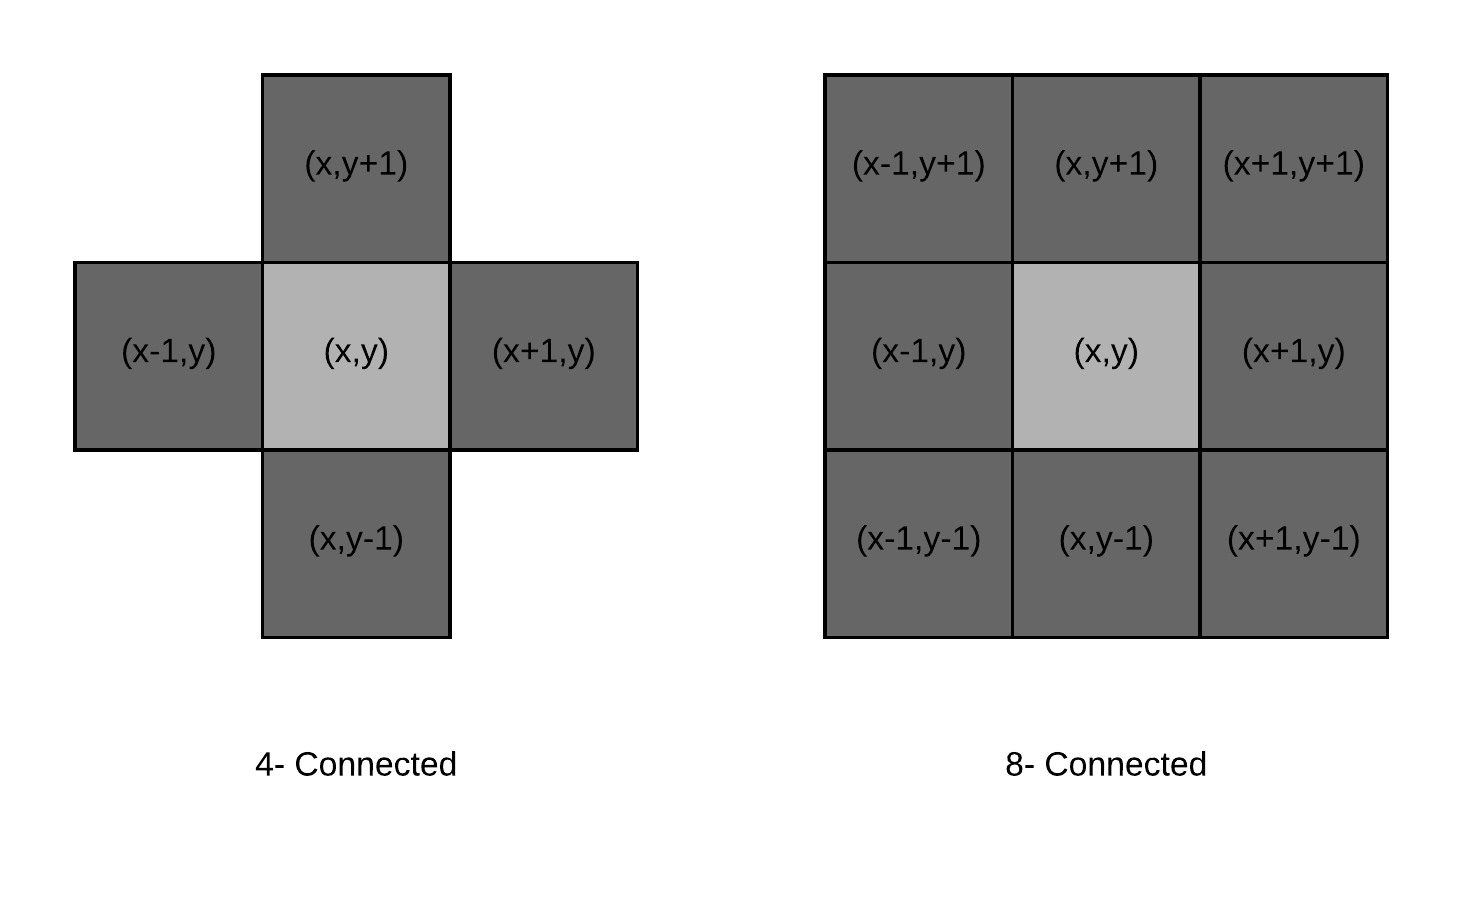
\includegraphics[width = 0.8\textwidth]{litreview/contours/connectedness.png}
    \caption{4- (8-) Connectedness of a pixel (x,y)}
    \label{fig:connectedness}
  \end{figure}

  \begin{figure}[H]
    \centering
    \centering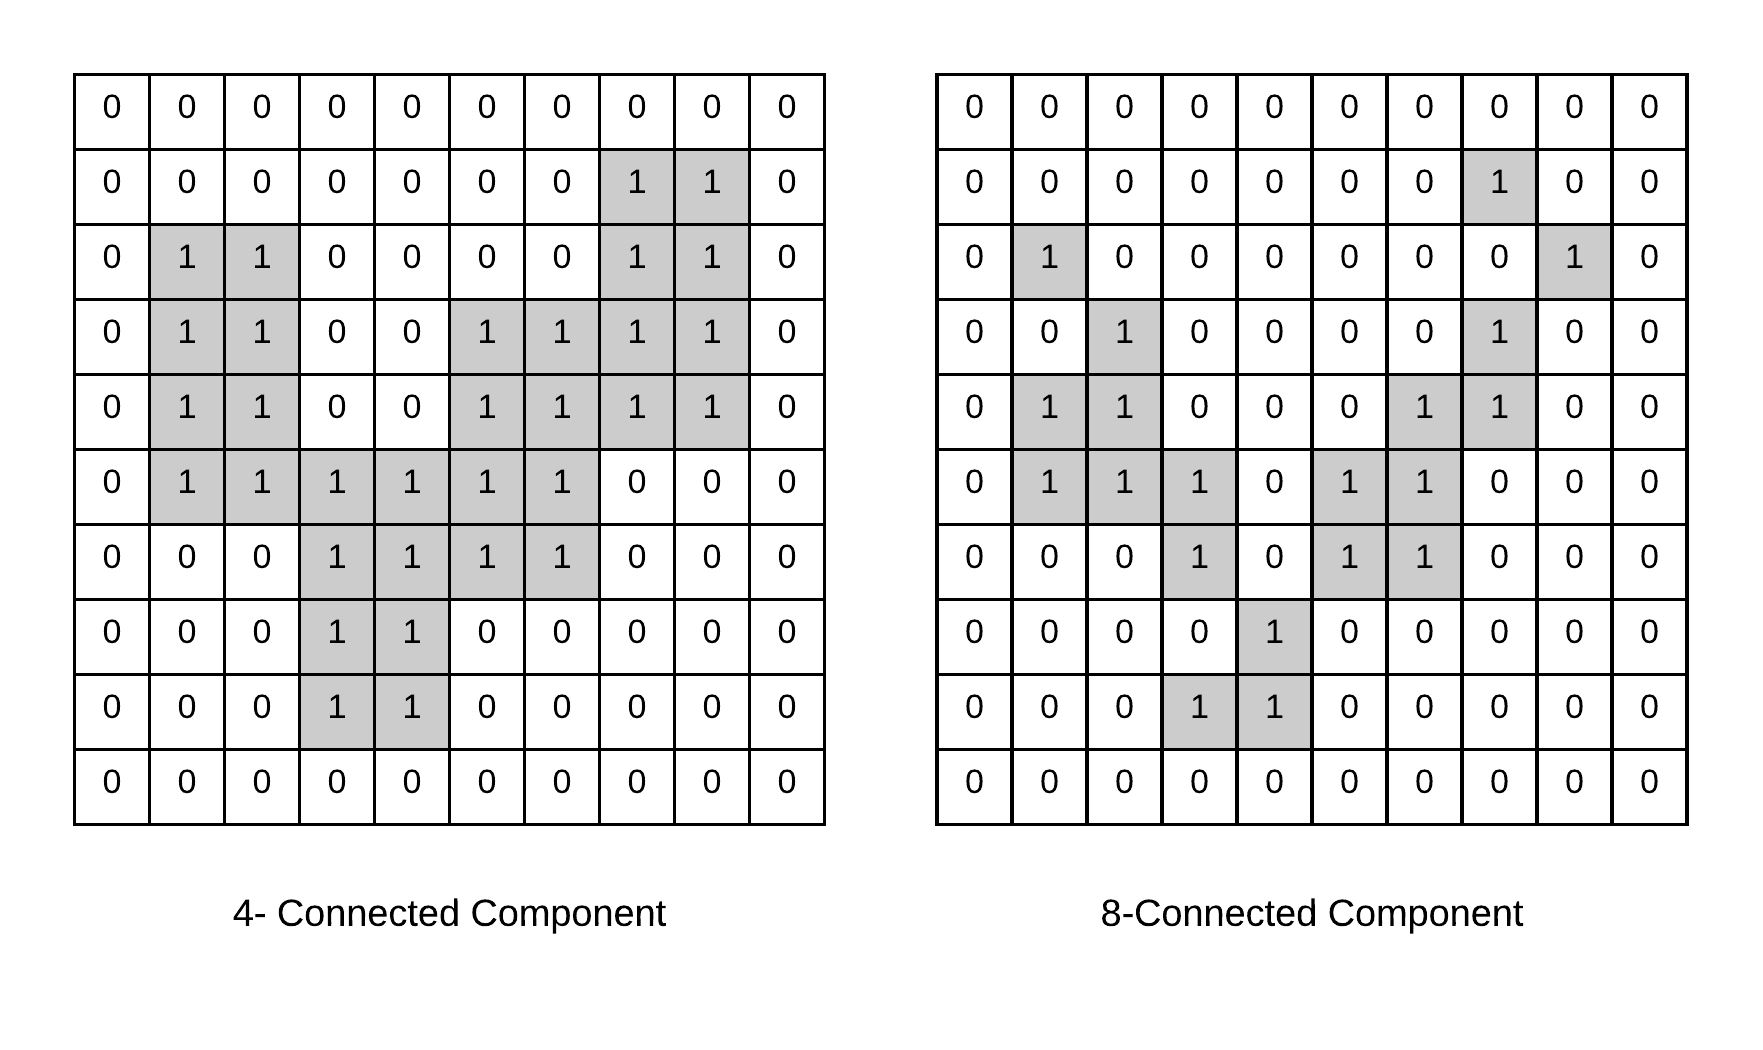
\includegraphics[width = 0.8\textwidth]{litreview/contours/connection_examples}
    \caption{Examples of different types of connected components.}
    \label{fig:connection_examples}
  \end{figure}
  

When the algorithm is performed the cells of the image are scanned in a raster fashion (left to right, top to bottom) and when a 1-pixel is encountered the algorithm interrupts and determines the type of border the pixel is that it ran into to. There are two types of border a hole border and an outer border. Figure \ref{fig:borders} illustrates these two types of borders. Satoshi defines a border point to be one that has a 0-pixel in its 4- (8-) neighborhood. An outer border is one surrounded by 0-pixel connected component and a hole border is one that surrounds a 0-pixel component. If a border is has thickness of only one pixel and is satisfies both being an outer border and hole border it's regarded as an outer border. The high-level outline of the algorithm is specified in Algorithm \ref{algorithm:satoshi} though the source material \cite{satoshi_findContours} should be consulted for a more comprehensive description.

\begin{figure}[H]
    \centering
    \centering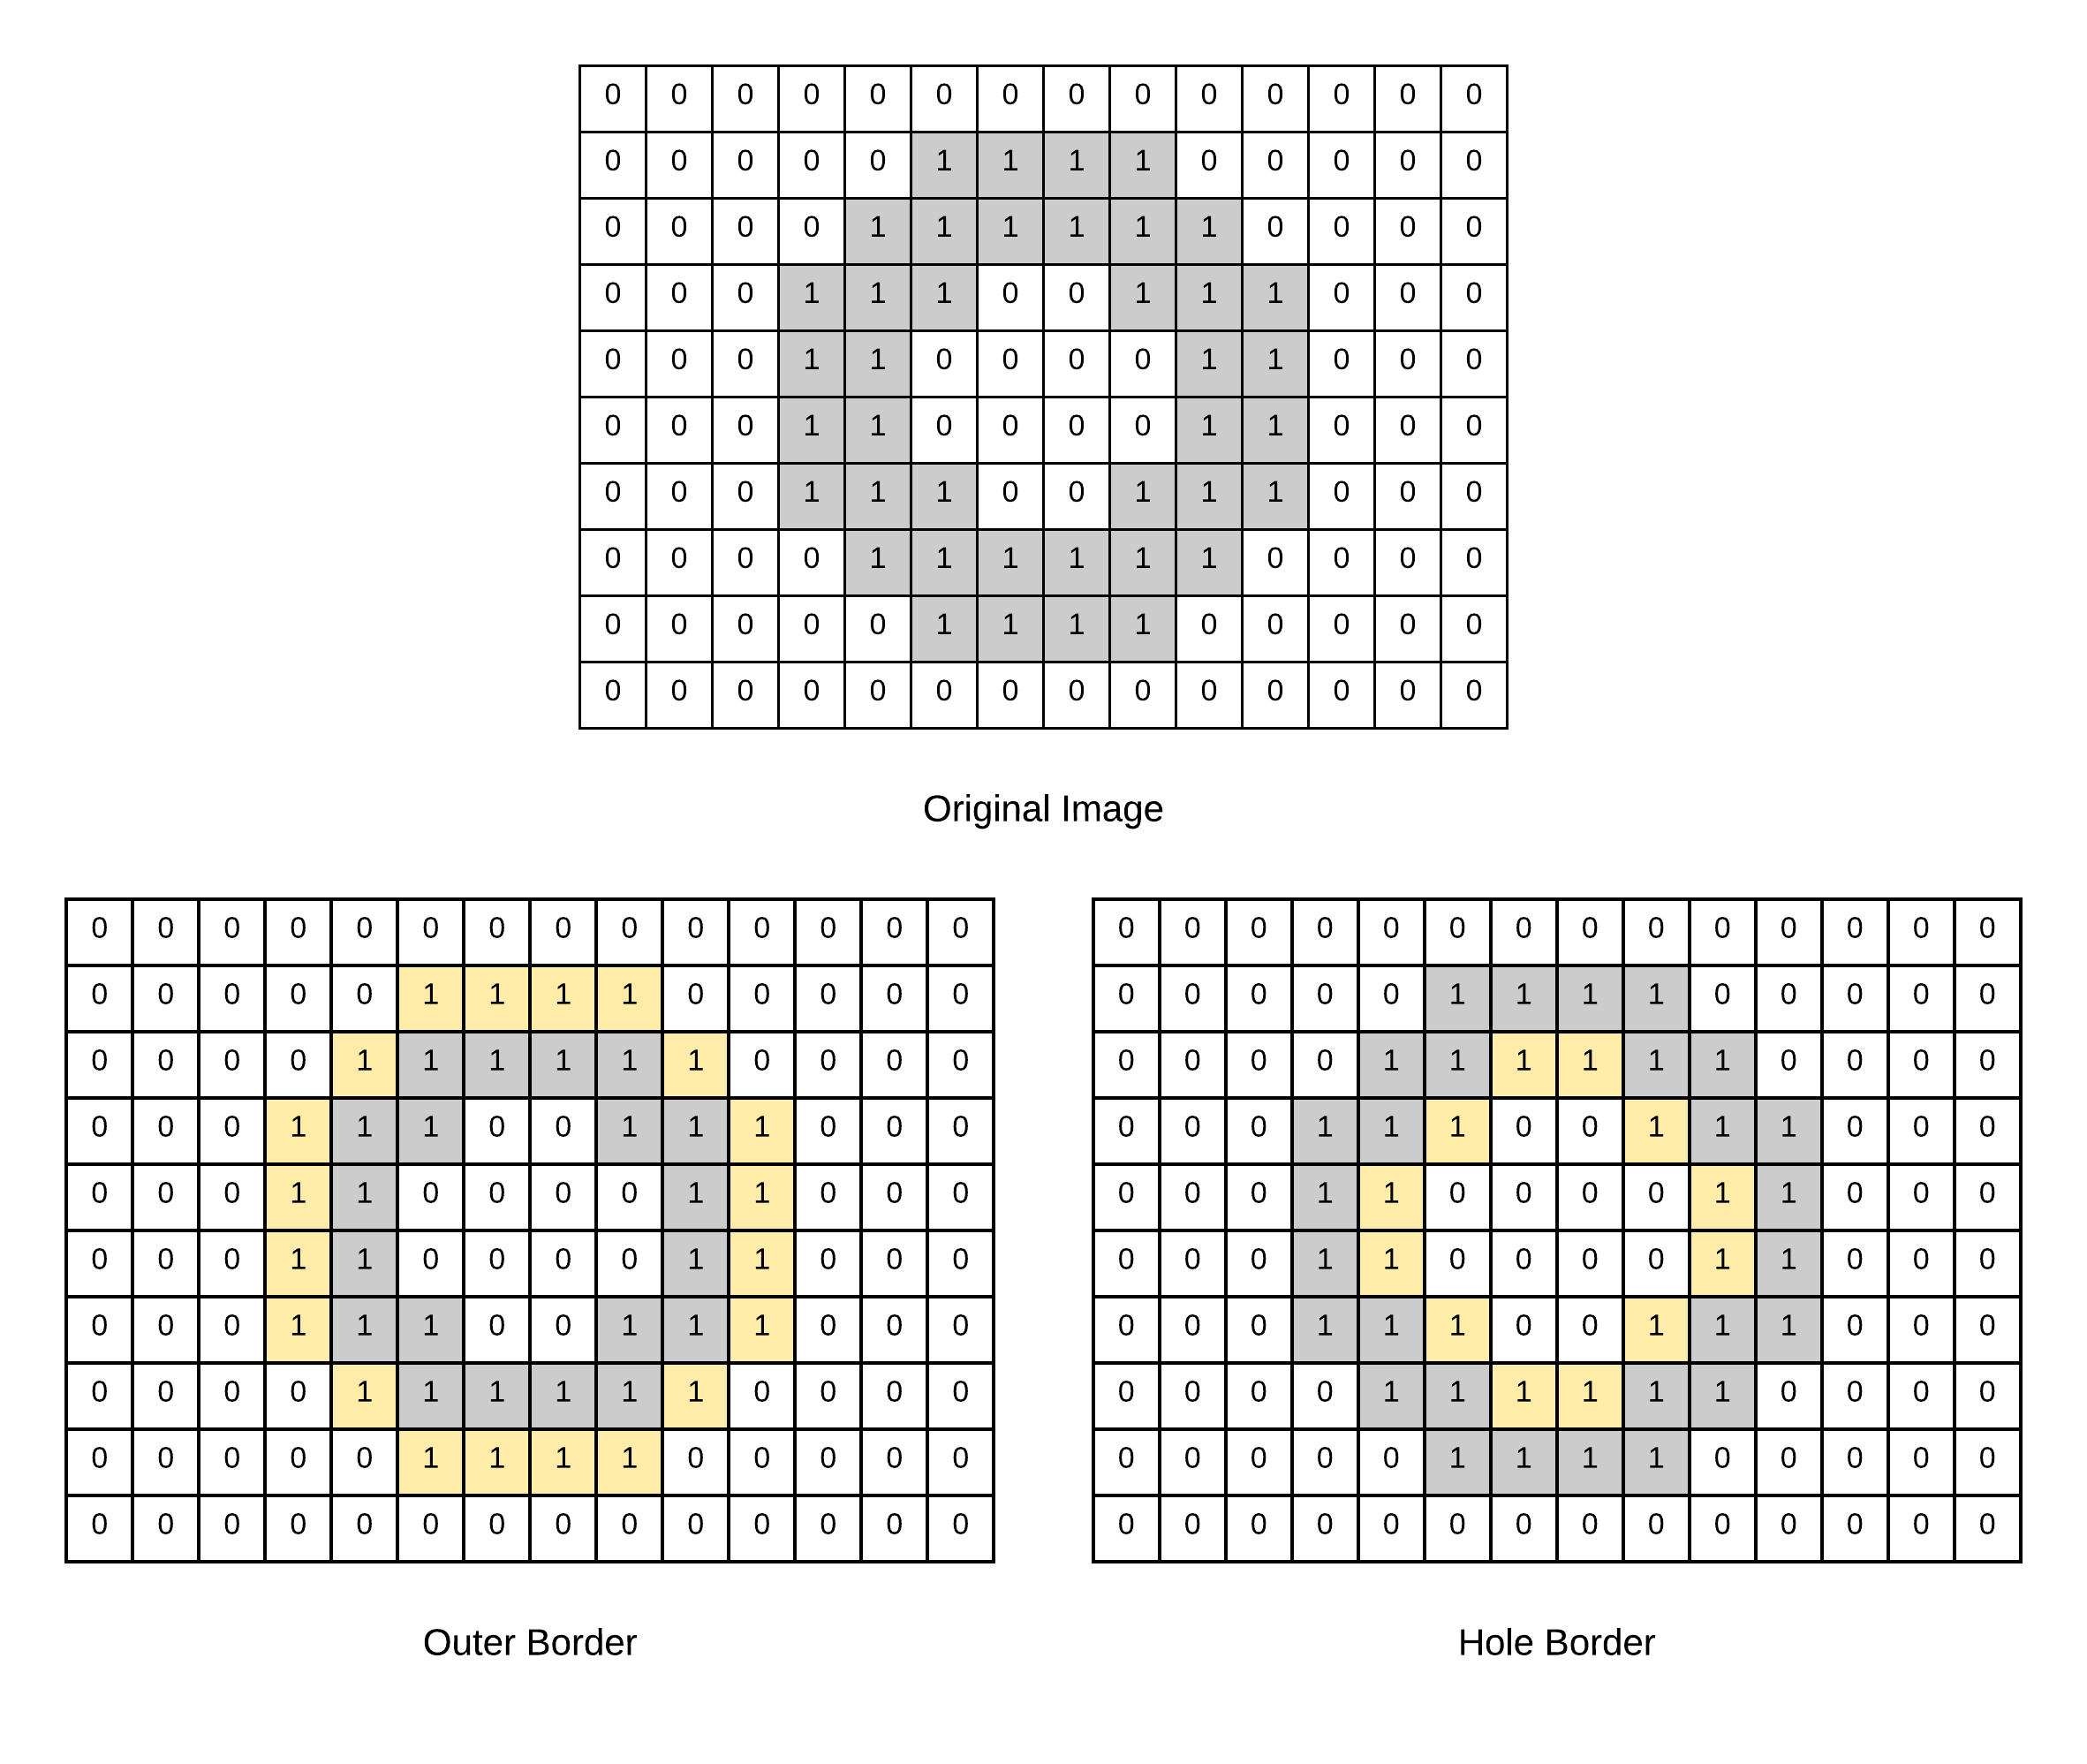
\includegraphics[width = 0.8\textwidth]{litreview/contours/borders}
    \caption{Comparison of a hole border and outer border.}
    \label{fig:borders}
  \end{figure}


\begin{algorithm}
\SetAlgoLined
\KwInput{Binary image, F, size I x J} 
\KwOutput{Coordinates of all object borders in F}
Initialize LNBM = 1 which tracks most recently labelled border.\;
Initialize counter NBD = 0 which tracks the number of borders created.\;
\While{imageScanner $\neq$ F[I,J]}{
    \uIf{F[i,j] = 1 and F[i,j-1] = 0}{
        F[i,j] is the starting point of an outer border\;
        follow border until return to starting point labelling all points with a unique ID\;
    }\uElseIf{F[i,j] $\geq$ 1 and F[i,j+1] = 0}{
        F[i,j] is the starting point of a hole border\;
        follow border until return to starting point labelling all points with a unique ID\;
    }
}
\caption{Satoshi Suzuki's algorithm for border tracing \cite{satoshi_findContours}.}
\label{algorithm:satoshi}
\end{algorithm}


  


\subsection{Tracking}

The tracking component of the detection algorithm takes a list of bounding box coordinates corresponding to each foreground object and generates tracked objects that contain the coordinates history of the objects. 

Each vehicle object's location in an image is represented by the centre of its bounding box, called a centroid, by maintaining a history of an object's centroid position over time its path can be tracked through the video. For each image new centroids are recalculated for every object and by comparing the new centroid locations with the old centroid locations the new position of objects can be determined. New centroids are assigned to the objects whose last known position was closest. Algorithm \ref{algorithm:centroid_reassign} outlines the centroid reassignment process.

\begin{algorithm}
  \SetAlgoLined
  \KwInput{List of current centroids \emph{cen\_old}, size X, List of new centroids \emph{cen\_new}, size Y} 
  \KwOutput{Updated list of current centroids}
  Generate an $X \times Y$ distance matrix, $D$, between \emph{cen\_old} and \emph{cen\_new}\;
  Generate a list of column indices, \emph{cols} from $D$ sorted by the column containing the smallest value to the largest\;
  Generate a list of row indices, \emph{rows}, from $D$ corresponding to the row containing the smallest values in \emph{cols}.\;
  \For{(i,j) in (\emph{rows}, \emph{cols})}{
    \If{cen\_new[j] not used and cen\_old[i] not used}{
        \emph{cen\_old[i]} = \emph{cen\_new[j]}\;
        mark \emph{cen\_old[i]} as used\;
        mark \emph{cen\_new[j]} as used\;
    }
  }
  \For{\emph{cen} in unused \emph{cen\_new}}{
    \emph{cen\_old}.append(\emph{cen})\;
  }
  \For{\emph{cen} in unused \emph{cen\_old}}{
    mark \emph{cen} as missing\;
  }
  \caption{Centroid re-assignment algorithm. \cite{adrian_rosebrock_simple_object_tracking}}
  \label{algorithm:centroid_reassign}
\end{algorithm}

If a new position cannot be found for an object then it has a limited number of frames it can be missing for before it's removed, objects generally go missing due to partial or complete occlusion by other vehicles, alternatively they will go missing permanently if they leave the node's field of view. Vehicle's can also disappear if they remain stationery long enough to be considered background pixels by the subtractor. Figure \ref{fig:centroids} visualizes the centroids on the objects along with a unique identifier which is used to mark ownership of a foreground object. Notice in Figure \ref{fig:centroids} centroids 25 and 24 belong to no object, this is because they have not yet timed out, meaning their object hasn't been missing from frame long enough for them to be dismissed, this is also the case for centroid 16. Centroids 1 and 9 belong to a cluster of vehicles that have become distant (see Figure \ref{fig:original_frame}), this occurs because as the vehicles travel further away the distance between them in pixels becomes less and so the morphological process presses them together. This is not an issue if the counting and measuring system is calibrated to focus on areas where vehicles are easily separable. 

\begin{figure}[H]
    \centering
    \centering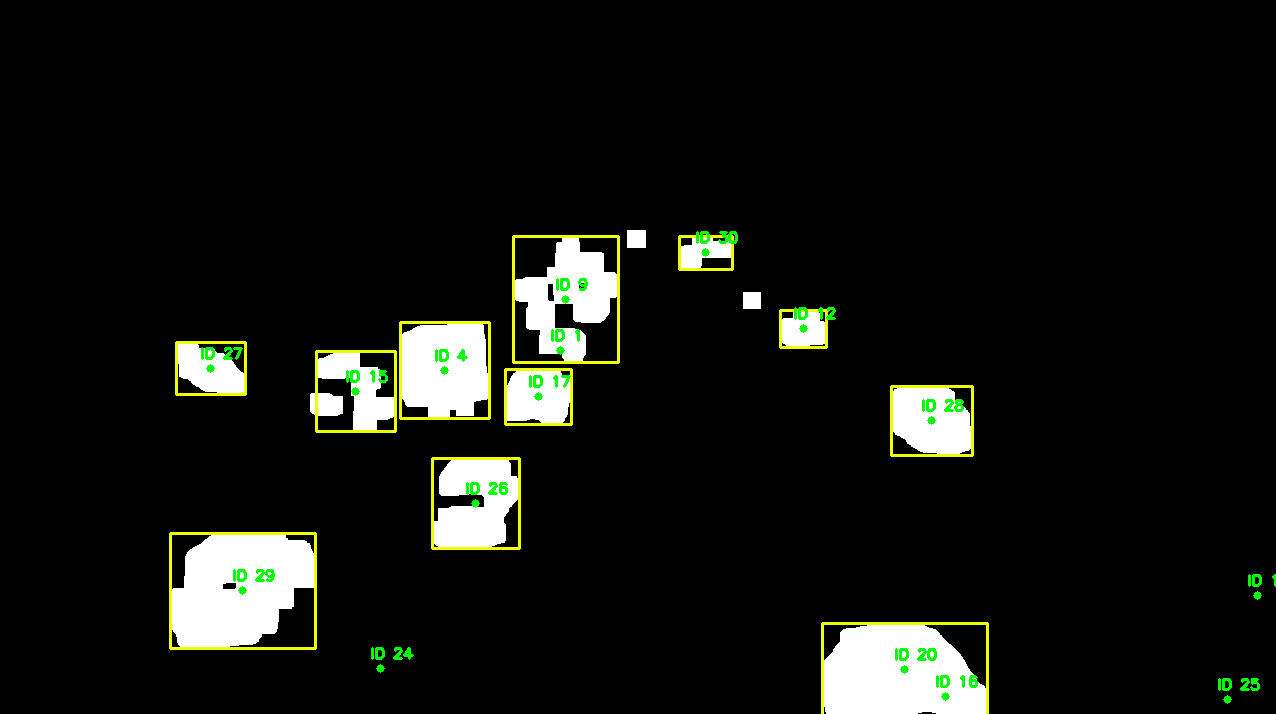
\includegraphics[width = 0.8\textwidth]{design/detection/tracking/mask_centroids}
    \caption{Centroids plotted over foreground objects.}
    \label{fig:centroids}
\end{figure}

\subsubsection{Calibration}

For a given traffic scenario we seek to set a maximum\_distance and minimum\_distance which control centroid reassignment. We also should consider the amount of time a object can go missing for. 

The minimum\_distance parameter addresses failure of the morphology component of the algorithm to recombine some blobs. After all centroids are reassigned an additional consolidation process is performed where if any two centroids are closer together than min\_distance they are merged into a single centroid. Figure \ref{fig:centroids_consolidation} compares two centroid allocations for the same image where one performs centroid combination and the other doesn't. In Figure \ref{fig:consolidateA} the number of centroids is greater thus consuming more computational power and increasing the number of false positive counts.

Maximum\_distance controls the allowed distance a new centroid can be from an old one and still be considered its new position. In cases where there are more new centroids than old ones, without this parameter restriction, centroid allocations will store an old centroid's an unreasonable distance from its old position when in reality a new centroid should be generated and not reassignment performed.

The second calibration consideration for tracking is how long the system allows an object to be missing. Determination of this quantity dependent on how frequently vehicles are occluded and for how long. In a situation where there was an obstacle consistently blocking vision of the road for a period then the amount of time a centroid should be stored is proportional to how long a vehicle is occluded by that obstacle on average. Its common that an object may disappear for a few frames so it's important for objects to be able to go missing and remerge else lots of data could be lost.

\begin{figure}[H]
\centering
\begin{subfigure}[b]{0.45\linewidth}
            \centering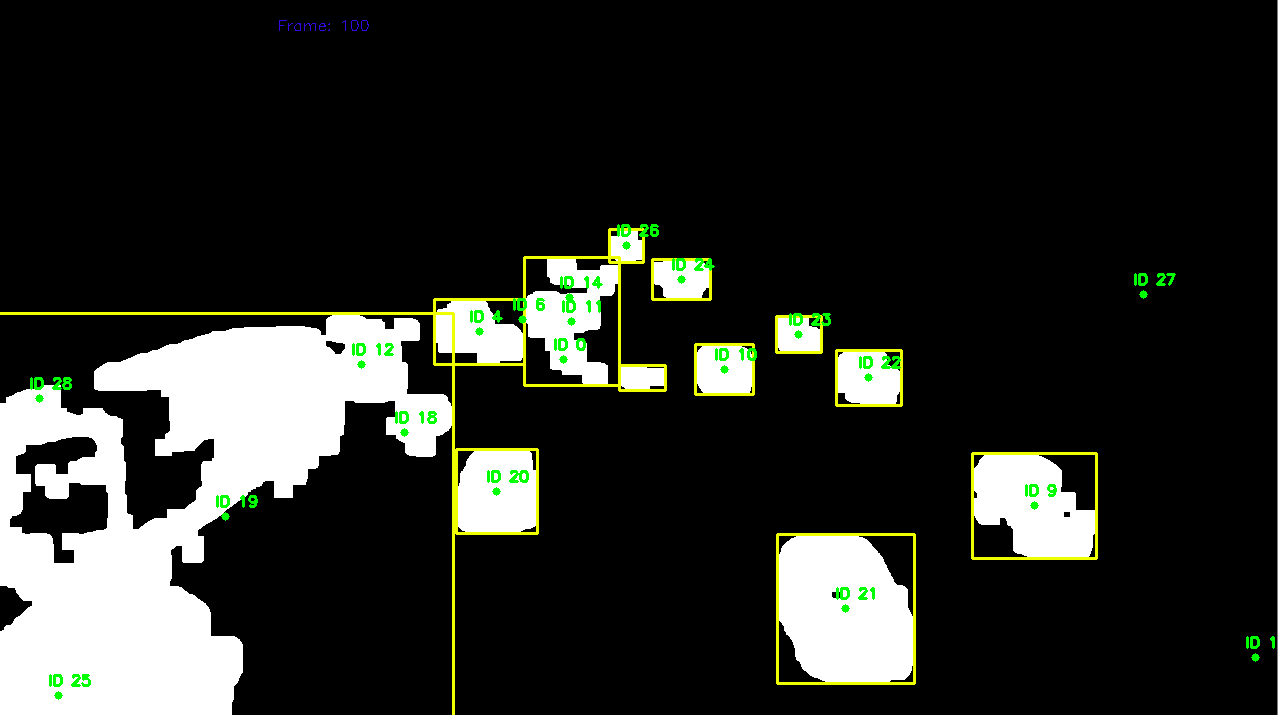
\includegraphics[width = \textwidth]{design/detection/calibration/mask_noconsolidate}
            \captionsetup{format=hang}
            \caption{Centroid tracking with no consolidation distance set (16 centroids).}
            \label{fig:consolidateA}
  \label{fig:}
    \end{subfigure}
    \begin{subfigure}[b]{0.45\linewidth}
            \centering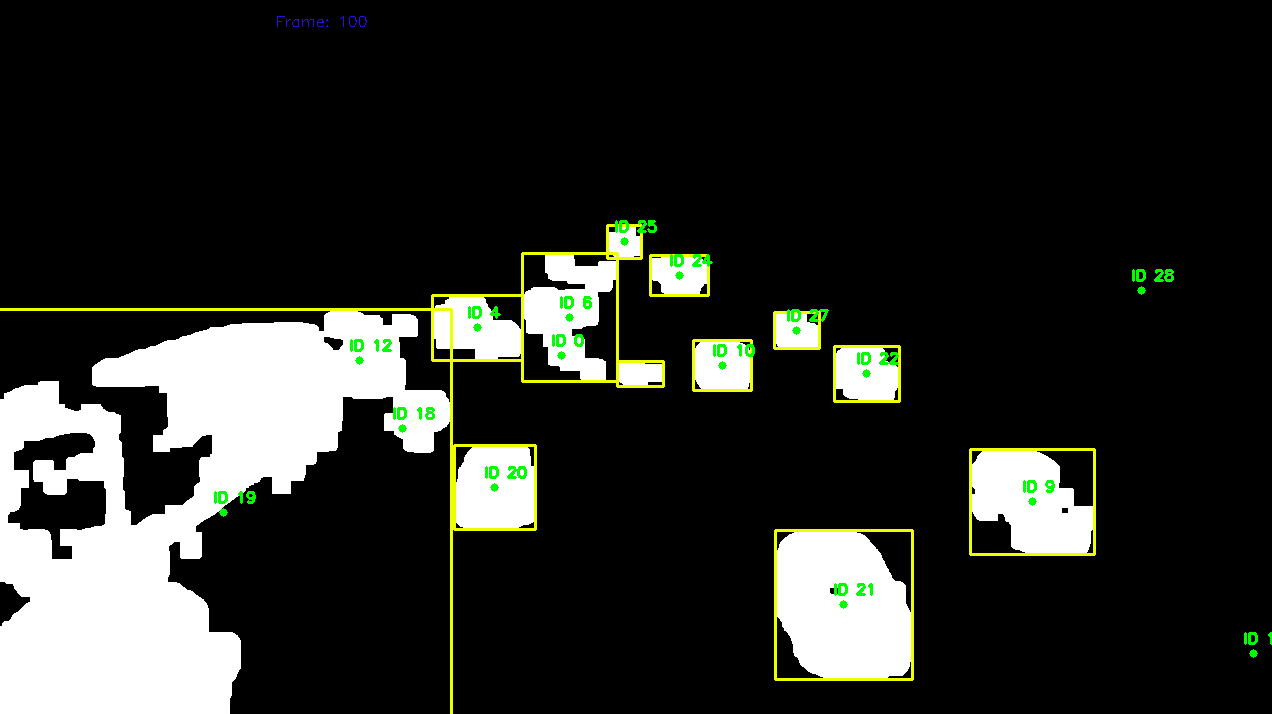
\includegraphics[width = \textwidth]{design/detection/calibration/mask_consolidate}
            \captionsetup{format=hang}
        \caption{Centroid tracking with consolidation distance set (20 centroids).}
        \label{fig:consolidateB}
      \end{subfigure}
      \captionsetup{format=hang}
    \caption{Comparison of centroid generation with and without consolidating centroids based on distance.}
    \label{fig:centroids_consolidation}
\end{figure}
  


